\documentclass[12pt, a4paper]{article}

% ─── Packages ────────────────────────────────────────────────────────────────
\usepackage[T1]{fontenc}
\usepackage[utf8]{inputenc}
\usepackage[margin=2.5cm, top=3cm, bottom=3cm]{geometry}
\usepackage{xcolor}
\usepackage{titlesec}
\usepackage{titling}
\usepackage{fancyhdr}
\usepackage{booktabs}
\usepackage{array}
\usepackage{tabularx}
\usepackage{colortbl}
\usepackage{amsmath}
\usepackage{amssymb}
\usepackage{graphicx}
\usepackage{hyperref}
\usepackage{parskip}
\usepackage{enumitem}
\usepackage{tcolorbox}
\usepackage{mdframed}
\usepackage{listings}
\usepackage{caption}
\usepackage{subcaption}
\usepackage{float}
\usepackage{setspace}
\usepackage{tikz}
\usepackage{multirow}
\usepackage{longtable}
\usetikzlibrary{shapes.geometric, arrows.meta, positioning, fit, backgrounds, calc, shadows}

% ─── Color Palette ────────────────────────────────────────────────────────────
\definecolor{primary}{RGB}{31, 73, 125}
\definecolor{secondary}{RGB}{0, 112, 192}
\definecolor{accent}{RGB}{192, 0, 0}
\definecolor{lightblue}{RGB}{219, 233, 246}
\definecolor{lightgray}{RGB}{245, 245, 245}
\definecolor{darkgray}{RGB}{64, 64, 64}
\definecolor{medgray}{RGB}{130, 130, 130}
\definecolor{tablehead}{RGB}{31, 73, 125}
\definecolor{rulecolor}{RGB}{0, 112, 192}
\definecolor{codebg}{RGB}{248, 249, 250}
\definecolor{noteboxbg}{RGB}{255, 248, 230}
\definecolor{noteborder}{RGB}{200, 150, 0}
\definecolor{warningbg}{RGB}{253, 236, 234}
\definecolor{warningborder}{RGB}{192, 0, 0}
\definecolor{webgreen}{RGB}{0, 128, 80}
\definecolor{webbg}{RGB}{230, 247, 238}
\definecolor{successgreen}{RGB}{34, 139, 34}
% TikZ node colors
\definecolor{tikzblue}{RGB}{31, 73, 125}
\definecolor{tikzlightblue}{RGB}{180, 210, 240}
\definecolor{tikzgreen}{RGB}{0, 128, 80}
\definecolor{tikzlightgreen}{RGB}{200, 235, 215}
\definecolor{tikzred}{RGB}{192, 0, 0}
\definecolor{tikzlightred}{RGB}{250, 215, 215}
\definecolor{tikzgold}{RGB}{180, 130, 0}
\definecolor{tikzlightgold}{RGB}{255, 245, 200}
\definecolor{tikzgray}{RGB}{90, 90, 90}
\definecolor{tikzlightgray}{RGB}{235, 235, 235}

% ─── Graphics path ────────────────────────────────────────────────────────────
\graphicspath{{report_images/}}

% ─── Hyperref setup ───────────────────────────────────────────────────────────
\hypersetup{
  colorlinks=true,
  linkcolor=secondary,
  citecolor=primary,
  urlcolor=secondary,
  pdftitle={Multilingual RAG Chatbot -- Architecture, Implementation, and Evaluation},
  pdfauthor={Bettayeb Mohamed Aimen, Amina, Yanis, Loubna},
}

% ─── Section Styling ──────────────────────────────────────────────────────────
\titleformat{\section}
  {\color{primary}\large\bfseries}
  {\color{secondary}\thesection.}{0.6em}{}
  [\vspace{-0.3em}\color{rulecolor}\rule{\linewidth}{0.8pt}\vspace{0.3em}]

\titleformat{\subsection}
  {\color{primary}\normalsize\bfseries}
  {\color{secondary}\thesubsection}{0.6em}{}

\titleformat{\subsubsection}
  {\color{darkgray}\normalsize\itshape}
  {\thesubsubsection}{0.5em}{}

\titlespacing{\section}{0pt}{1.4em}{0.6em}
\titlespacing{\subsection}{0pt}{1em}{0.4em}

% ─── Header / Footer ─────────────────────────────────────────────────────────
\pagestyle{fancy}
\fancyhf{}
\renewcommand{\headrulewidth}{0pt}
\fancyhead[L]{\small\color{medgray}\textit{Multilingual RAG Chatbot --- Architecture, Implementation, and Evaluation}}
\fancyhead[R]{\small\color{medgray}\thepage}
\fancyfoot[C]{\color{medgray}\rule{0.3\linewidth}{0.4pt}}

% ─── Table styling ───────────────────────────────────────────────────────────
\renewcommand{\arraystretch}{1.4}
\newcolumntype{L}[1]{>{\raggedright\arraybackslash}p{#1}}
\newcolumntype{C}[1]{>{\centering\arraybackslash}p{#1}}

% ─── tcolorbox environments ───────────────────────────────────────────────────
\tcbuselibrary{skins, breakable}

\newtcolorbox{notebox}{
  colback=noteboxbg, colframe=noteborder,
  fonttitle=\bfseries\small\color{white},
  title={\small Design Rationale},
  arc=3pt, boxrule=0.8pt,
  left=8pt, right=8pt, top=6pt, bottom=6pt, breakable
}

\newtcolorbox{warningbox}{
  colback=warningbg, colframe=warningborder,
  fonttitle=\bfseries\small\color{white},
  title={\small Safety Principle},
  arc=3pt, boxrule=0.8pt,
  left=8pt, right=8pt, top=6pt, bottom=6pt, breakable
}

\newtcolorbox{failurebox}{
  colback=lightgray, colframe=medgray,
  fonttitle=\bfseries\small,
  title={\small Failure Case},
  arc=3pt, boxrule=0.6pt,
  left=8pt, right=8pt, top=6pt, bottom=6pt, breakable
}

\newtcolorbox{webbox}{
  colback=webbg, colframe=webgreen,
  fonttitle=\bfseries\small\color{white},
  title={\small Web Search Note},
  arc=3pt, boxrule=0.8pt,
  left=8pt, right=8pt, top=6pt, bottom=6pt, breakable
}

% ─── Listings ────────────────────────────────────────────────────────────────
\lstset{
  backgroundcolor=\color{codebg},
  basicstyle=\small\ttfamily\color{darkgray},
  keywordstyle=\bfseries\color{primary},
  commentstyle=\itshape\color{medgray},
  frame=single, framerule=0.6pt,
  rulecolor=\color{rulecolor},
  xleftmargin=12pt, xrightmargin=6pt,
  breaklines=true,
  numbers=left, numberstyle=\tiny\color{medgray}, numbersep=8pt,
  tabsize=2, captionpos=b,
}

% ─── Misc ─────────────────────────────────────────────────────────────────────
\setstretch{1.15}
\setlength{\parindent}{0pt}
\setlength{\parskip}{0.55em}
\captionsetup{font=small, labelfont={bf,color=primary}, textfont=it}

% ─── TikZ arrow style ─────────────────────────────────────────────────────────
\tikzset{
  pipenode/.style={
    rectangle, rounded corners=4pt,
    minimum width=3.8cm, minimum height=0.7cm,
    text centered, font=\small\bfseries,
    draw=#1!80!black, fill=#1!20, text=black,
    drop shadow={shadow xshift=0.5pt, shadow yshift=-0.5pt, fill=black!15}
  },
  sourcebox/.style={
    rectangle, rounded corners=4pt,
    minimum width=3.2cm, minimum height=0.65cm,
    text centered, font=\small,
    draw=#1!80!black, fill=#1!15, text=black
  },
  pipe/.style={-{Stealth[length=5pt]}, thick, color=#1},
  dasharrow/.style={-{Stealth[length=4pt]}, dashed, thick, color=#1},
}

% ══════════════════════════════════════════════════════════════════════════════
\begin{document}

% ─── Title Page ───────────────────────────────────────────────────────────────
\begin{titlepage}
  \pagecolor{primary}
  \color{white}\centering
  \vspace*{2.5cm}
  {\fontsize{11}{13}\selectfont\color{lightblue}\MakeUppercase{Technical Research Report}}\\[0.4cm]
  \color{white}\rule{0.5\linewidth}{0.6pt}\\[1.2cm]
  {\fontsize{22}{27}\selectfont\bfseries
    A Multilingual RAG Chatbot\\[0.25em]
    for Arabic NLP and\\[0.25em]
    Legal Advisory}\\[1.0cm]
  \color{lightblue}\rule{0.4\linewidth}{0.4pt}\\[0.8cm]
  {\normalsize\itshape Architecture, Implementation, and Evaluation}\\[2.5cm]
  {\small
    \begin{tabular}{c}
      \textbf{Bettayeb Mohamed Aimen} \quad \textbf{Amina} \quad \textbf{Yanis} \quad \textbf{Loubna}\\[0.4em]
      \color{lightblue}Supervised by Mme Berkani
    \end{tabular}
  }\\[1.8cm]
  \color{lightblue}\rule{0.3\linewidth}{0.3pt}\\[0.5cm]
  {\small April 2026}
  \vfill
  {\footnotesize\color{medgray} Multilingual RAG Chatbot --- Architecture, Implementation, and Evaluation}
\end{titlepage}
\nopagecolor

% ─── Abstract ─────────────────────────────────────────────────────────────────
\newpage
\begin{abstract}
This report presents the design, implementation, and evaluation of a multilingual
Retrieval-Augmented Generation (RAG) chatbot built for the Arabic NLP Platform.
The system supports three languages (Arabic, French, English) across four
operational modes: Normal Chat, NLP \& AI research, Legal Advisory, and Platform
Guide. The architecture combines a 12-stage processing pipeline---from language
detection through faithfulness verification---with a hybrid retrieval engine
that fuses dense semantic search (BGE-M3 embeddings, Qdrant) and sparse lexical
search (BM25) using Reciprocal Rank Fusion (RRF).

We document the full conception-to-deployment lifecycle, including: (i)~a
theoretical framework covering transformer embeddings, BM25 scoring, RRF
fusion, and BERTScore evaluation; (ii)~the knowledge-base ingestion pipeline
using Docling for structure-aware PDF/XML parsing of 26~academic and legal
documents; (iii)~the migration from Groq (LLaMA-based) to Google Gemini as the
primary LLM provider due to hallucination issues in the legal domain; and
(iv)~a dual-channel web search system (Exa for automatic fallback, Tavily for
user-triggered search).

Automated evaluation demonstrates strong retrieval performance on the primary benchmark run (Section~14): Precision@5 of 0.7524, Recall@5 of 0.9405, and Mean Reciprocal Rank (MRR) of 0.8786, alongside semantic generation quality with BERTScore F1 of 0.9472. The run log explicitly records zero failures for this benchmark configuration. A dedicated human evaluation platform, deployed as a Next.js web application, enables domain-expert assessment across five criteria per domain (Legal, NLP, Web).
\end{abstract}

% ─── Table of Contents ────────────────────────────────────────────────────────
\newpage
\tableofcontents
\newpage

% ══════════════════════════════════════════════════════════════════════════════
%  SECTION 1 — INTRODUCTION
% ══════════════════════════════════════════════════════════════════════════════
\section{Introduction}

The rapid growth of Arabic Natural Language Processing (NLP) research, combined
with the increasing digitisation of legal texts across the MENA region, has
created a pressing need for intelligent systems capable of navigating
multilingual knowledge bases with high precision. Traditional keyword-based
search engines fall short when users pose complex, context-dependent questions
in Arabic, French, or English---particularly when the domain demands factual
accuracy, such as in legal advisory.

This report presents a comprehensive multilingual chatbot built on the
Retrieval-Augmented Generation (RAG) paradigm. The system is deployed as part
of an Arabic NLP research platform and serves four distinct operational modes:

\begin{enumerate}[leftmargin=2em]
  \item \textbf{Normal Chat} --- general conversational AI with guardrails.
  \item \textbf{NLP \& AI} --- retrieval over a curated corpus of 18~academic
        papers covering transformers, Arabic LLMs, and RAG systems.
  \item \textbf{Legal Advisor} --- retrieval over 8~Algerian legal
        documents (journal officiel, data protection laws, research ethics).
  \item \textbf{Platform Guide} --- structured search over platform entities
        (tools, courses, corpora, institutions) via PostgreSQL and
        Elasticsearch.
\end{enumerate}

The chatbot's architecture is distinguished by several design decisions:
\begin{itemize}[leftmargin=2em]
  \item A \textbf{hybrid retrieval engine} combining dense (BGE-M3) and sparse
        (BM25) search with Reciprocal Rank Fusion (RRF), eliminating the need
        for manual weight tuning.
  \item A \textbf{faithfulness verification gate} that uses a secondary LLM
        call to detect hallucinated legal provisions before they reach the user.
  \item A \textbf{dual LLM provider architecture} (Gemini primary, Groq
        fallback) that ensures high availability and allows provider-specific
        optimisation.
  \item A \textbf{structure-aware document ingestion} pipeline using Docling
        for section-level chunking of PDF and XML academic papers.
  \item A \textbf{dedicated human evaluation platform} deployed for
        researcher-led quality assessment across Legal, NLP, and Web domains.
\end{itemize}

The remainder of this report is organised as follows: Section~2 surveys related
work; Section~3 presents the theoretical background; Section~4 describes the
conception phase; Section~5 details the system architecture; Section~6 walks
through the methodology; Section~7 narrates the full journey of a query;
Sections~8--10 cover web search, document ingestion with Docling, and document
processing; Section~11 discusses the LLM provider migration; Section~12
presents the realisation; Section~13 provides comprehensive evaluation results;
Section~14 discusses findings; and Section~15 concludes.


% ══════════════════════════════════════════════════════════════════════════════
%  SECTION 2 — RELATED WORK
% ══════════════════════════════════════════════════════════════════════════════
\section{Related Work}

\subsection{Retrieval-Augmented Generation}
Lewis et al.~\cite{lewis2020rag} introduced RAG as a paradigm that
conditions language-model generation on documents retrieved from an external
knowledge store. This approach mitigates hallucination by grounding the
model's output in verifiable sources. Subsequent work by Gao et
al.~\cite{gao2024ragsurvey} surveyed the rapidly growing RAG landscape,
identifying hybrid retrieval and faithfulness verification as key open
challenges---both of which our system addresses.

\subsection{Hybrid Retrieval}
Combining semantic (dense) and lexical (sparse) retrieval has consistently
outperformed either method alone. Cormack et al.~\cite{cormack2009rrf}
proposed Reciprocal Rank Fusion (RRF), a simple, parameter-free method
for combining multiple ranked lists. Ma et al.~\cite{ma2024bm25rrf} demonstrated
that BM25 + dense retrieval with RRF achieves state-of-the-art performance on
multilingual benchmarks, motivating our adoption of this exact combination.

\subsection{Multilingual Embeddings}
Chen et al.~\cite{chen2024bgem3} introduced BGE-M3, a multi-lingual,
multi-functionality embedding model supporting over 100 languages. BGE-M3
simultaneously produces dense, sparse, and ColBERT-style embeddings within a
single forward pass. Its strong Arabic coverage and 8192-token context window
make it ideal for our multilingual legal and NLP knowledge base.

\subsection{Passage Reranking}
Cross-encoder reranking after initial retrieval has been shown to significantly
improve precision~\cite{nogueira2019passage}. Our system implements a
lightweight cosine-similarity reranker using BGE-M3 re-encoding, which
avoids the computational cost of a dedicated cross-encoder while still
providing meaningful reordering of candidate passages.

\subsection{Legal and Domain-Specific NLP}
Chalkidis et al.~\cite{chalkidis2020legalbert} demonstrated the need for
domain-specific pretraining in legal NLP, achieving significant improvements
over general-purpose models. In the Arabic legal domain, the challenge is
compounded by the scarcity of digitised legal corpora and the coexistence
of Modern Standard Arabic with French in North African jurisdictions. Our
system addresses this by ingesting bilingual legal documents and applying
structure-aware chunking that preserves article boundaries.

\subsection{Faithfulness and Grounded Generation}
Honovich et al.~\cite{honovich2022true} proposed TRUE, a framework for
evaluating factual consistency between generated text and source documents.
In the legal domain, unfaithful generation can have real consequences---a
hallucinated article number or misquoted regulation could lead to incorrect
legal advice. Our faithfulness verification gate draws on this principle,
using a secondary LLM call with constrained output to classify each
response as \texttt{faithful} or \texttt{not\_faithful}.

\subsection{Web-Augmented Question Answering}
Lazaridou et al.~\cite{lazaridou2022internet} showed that augmenting LLMs
with live web retrieval improves factual accuracy on time-sensitive queries.
Our dual-channel approach (Exa for automatic semantic search, Tavily for
user-triggered keyword search) extends this concept with budget controls
and result caching to manage API costs.

\subsection{Evaluation of Generated Text}
Zhang et al.~\cite{zhang2020bertscore} introduced BERTScore, a metric that
leverages contextual embeddings to compute semantic similarity between
generated and reference texts. Unlike BLEU or ROUGE, BERTScore captures
paraphrastic equivalence, making it particularly suitable for evaluating
multilingual RAG systems where the generated answer may use different
phrasing than the reference.

\subsection{Document Processing and Ingestion}
Docling~\cite{docling2024} provides structure-aware PDF parsing that
preserves document hierarchy (sections, subsections, paragraphs) during
text extraction. This is critical for academic and legal documents where
section boundaries carry semantic meaning. The Hierarchical Chunker
produces chunks that respect section boundaries, improving retrieval
precision compared to na\"ive sliding-window approaches.

\subsection{Large Language Models}
Vaswani et al.~\cite{vaswani2017attention} introduced the Transformer
architecture that underpins all modern LLMs. The GPT family~\cite{brown2020gpt3}
demonstrated few-shot learning capabilities, while Google's Gemini
models~\cite{google2024gemini} advanced multilingual reasoning. In our
system, we migrated from Groq-hosted LLaMA models to Gemini due to
superior performance in Arabic legal contexts and reduced hallucination rates.


% ══════════════════════════════════════════════════════════════════════════════
%  SECTION 3 — THEORETICAL BACKGROUND
% ══════════════════════════════════════════════════════════════════════════════
\section{Theoretical Background}

This section presents the mathematical foundations underlying each component
of our RAG pipeline. Understanding these formulations is essential for
appreciating the design decisions documented in later sections.

\subsection{Transformer Architecture}

The Transformer~\cite{vaswani2017attention} replaces recurrent connections
with a self-attention mechanism that processes all positions in parallel.

\subsubsection{Scaled Dot-Product Attention}
Given queries $Q \in \mathbb{R}^{n \times d_k}$, keys $K \in \mathbb{R}^{m \times d_k}$,
and values $V \in \mathbb{R}^{m \times d_v}$, the attention function is:
\begin{equation}
  \text{Attention}(Q, K, V) = \text{softmax}\!\left(\frac{Q K^\top}{\sqrt{d_k}}\right) V
  \label{eq:attention}
\end{equation}
The scaling factor $\sqrt{d_k}$ prevents the dot products from growing
excessively large in high-dimensional spaces, which would push the softmax
into regions of vanishing gradients.

\subsubsection{Multi-Head Attention}
Rather than computing a single attention function, the Transformer applies
$h$ parallel attention heads:
\begin{equation}
  \text{MultiHead}(Q, K, V) = \text{Concat}(\text{head}_1, \ldots, \text{head}_h)\, W^O
\end{equation}
where $\text{head}_i = \text{Attention}(Q W_i^Q, K W_i^K, V W_i^V)$ and
$W_i^Q \in \mathbb{R}^{d_{\text{model}} \times d_k}$,
$W_i^K \in \mathbb{R}^{d_{\text{model}} \times d_k}$,
$W_i^V \in \mathbb{R}^{d_{\text{model}} \times d_v}$,
$W^O \in \mathbb{R}^{h d_v \times d_{\text{model}}}$.

\subsection{Dense Embeddings (BGE-M3)}

BGE-M3~\cite{chen2024bgem3} produces a fixed-dimensional vector
$\mathbf{e} \in \mathbb{R}^{1024}$ for each text passage. The similarity
between a query $q$ and a document $d$ is computed via cosine similarity:
\begin{equation}
  \text{sim}(q, d) = \frac{\mathbf{e}_q \cdot \mathbf{e}_d}{\|\mathbf{e}_q\| \, \|\mathbf{e}_d\|}
  \label{eq:cosine}
\end{equation}
In our system, Qdrant stores these vectors and performs approximate nearest
neighbour (ANN) search using HNSW indexing with an inner product metric.

\subsection{BM25 Sparse Retrieval}

BM25 (Best Matching 25)~\cite{robertson2009bm25} is a probabilistic ranking
function. For a query $Q$ containing terms $q_1, \ldots, q_n$ and a document
$D$, the BM25 score is:
\begin{equation}
  \text{BM25}(D, Q) = \sum_{i=1}^{n} \text{IDF}(q_i) \cdot
  \frac{f(q_i, D) \cdot (k_1 + 1)}{f(q_i, D) + k_1 \cdot \left(1 - b + b \cdot \frac{|D|}{\text{avgdl}}\right)}
  \label{eq:bm25}
\end{equation}
where:
\begin{itemize}[leftmargin=2em]
  \item $f(q_i, D)$ is the term frequency of $q_i$ in document $D$
  \item $|D|$ is the document length in tokens
  \item $\text{avgdl}$ is the average document length across the corpus
  \item $k_1 = 1.5$ controls term frequency saturation
  \item $b = 0.75$ controls document length normalisation
  \item $\text{IDF}(q_i) = \ln\!\left(\frac{N - n(q_i) + 0.5}{n(q_i) + 0.5} + 1\right)$
        is the inverse document frequency
\end{itemize}

Our BM25 implementation uses the \texttt{rank\_bm25} library with
\texttt{BM25Okapi} variant and a custom multilingual tokeniser that removes
stop words in Arabic, French, and English.

\subsection{Reciprocal Rank Fusion (RRF)}
\label{sec:rrf}

RRF~\cite{cormack2009rrf} combines multiple ranked lists without requiring
score normalisation or weight tuning. For a document $d$ appearing at rank
$r_i(d)$ in the $i$-th ranked list:
\begin{equation}
  \text{RRF}(d) = \sum_{i=1}^{L} \frac{1}{k + r_i(d)}
  \label{eq:rrf}
\end{equation}
where $k = 60$ is the fusion constant from the original paper. The constant
$k$ mitigates the impact of high rankings in a single list---a document ranked
1st in one list and absent from another receives $\frac{1}{61} \approx 0.0164$,
while a document ranked 1st in both lists receives $\frac{2}{61} \approx 0.0328$.

\begin{notebox}
We chose RRF over learned fusion methods (e.g., weighted linear combination)
because it is \textbf{parameter-free}---eliminating the need for a
held-out validation set to tune weights. This is critical in our setting
where the knowledge base spans multiple domains (NLP, legal, platform)
with different score distributions.
\end{notebox}

\subsection{Jaccard Similarity for Deduplication}

After fusion, near-duplicate documents are removed using word-set Jaccard
similarity:
\begin{equation}
  J(A, B) = \frac{|W_A \cap W_B|}{|W_A \cup W_B|}
  \label{eq:jaccard}
\end{equation}
where $W_A$ and $W_B$ are the sets of lowercased words in documents $A$ and
$B$. Documents with $J(A, B) \geq 0.85$ are considered near-duplicates.

\subsection{Cosine Reranking}

The top candidates after deduplication are re-scored by computing fresh
cosine similarity (Equation~\ref{eq:cosine}) between the query embedding
and a re-encoded version of each document's first 500 characters. This
second encoding pass provides a more accurate similarity estimate than
the initial ANN search, which uses approximate neighbours.

\subsection{BERTScore}
\label{sec:bertscore_theory}

BERTScore~\cite{zhang2020bertscore} evaluates semantic similarity between
a candidate sentence $\hat{x}$ and a reference sentence $x$ using
contextual embeddings from a pretrained language model. Let
$\hat{\mathbf{x}} = \langle \hat{\mathbf{x}}_1, \ldots, \hat{\mathbf{x}}_k \rangle$
and $\mathbf{x} = \langle \mathbf{x}_1, \ldots, \mathbf{x}_l \rangle$ be the
token embeddings.

\textbf{Precision} (how much of the candidate is supported by the reference):
\begin{equation}
  P_{\text{BERT}} = \frac{1}{|\hat{\mathbf{x}}|} \sum_{\hat{x}_j \in \hat{\mathbf{x}}}
  \max_{x_i \in \mathbf{x}} \hat{\mathbf{x}}_j^\top \mathbf{x}_i
  \label{eq:bertscore_p}
\end{equation}

\textbf{Recall} (how much of the reference is covered by the candidate):
\begin{equation}
  R_{\text{BERT}} = \frac{1}{|\mathbf{x}|} \sum_{x_i \in \mathbf{x}}
  \max_{\hat{x}_j \in \hat{\mathbf{x}}} \mathbf{x}_i^\top \hat{\mathbf{x}}_j
  \label{eq:bertscore_r}
\end{equation}

\textbf{F1 Score} (harmonic mean):
\begin{equation}
  F_{\text{BERT}} = 2 \cdot \frac{P_{\text{BERT}} \cdot R_{\text{BERT}}}{P_{\text{BERT}} + R_{\text{BERT}}}
  \label{eq:bertscore_f1}
\end{equation}

In our evaluation, we use the \texttt{microsoft/deberta-xlarge-mnli} model
as the backbone for BERTScore computation, which provides strong cross-lingual
semantic matching capabilities.

\subsection{LLM-based Ambiguity Resolution}
\label{sec:ambiguity_theory}

When the primary intent classifier (Section~\ref{sec:intent_class}) returns
a confidence score $C \leq 0.60$, the system enters an ambiguity resolution
phase. Theoretically, this is modeled as a \textbf{Meta-Reasoning} step.
Let $\mathcal{I} = \{i_1, i_2, \ldots, i_n\}$ be the set of possible intents.
The classifier produces a probability distribution $P(i|q)$. If the gap
between the top two candidates is small:
\begin{equation}
  P(i_{(1)}|q) - P(i_{(2)}|q) < \epsilon
\end{equation}
the system prompts a secondary LLM instance with the query $q$ and the
candidates $\{i_{(1)}, i_{(2)}\}$. The LLM acts as a high-reasoning judge
to resolve the semantic overlap, effectively applying domain-specific
knowledge that the embedding-based classifier might lack.

\subsection{Stateful RAG and Semantic Persistence}
\label{sec:stateful_rag}

To support fluid multi-turn conversations about specific documents, our
system implements a \textbf{Stateful RAG} paradigm. Unlike stateless
systems that re-classify every turn from scratch, we maintain a
document-mode state $S_t \in \{0, 1\}$.

The transition from $S_t = 1$ (Active Document Mode) to $S_t = 0$ is
governed by a \textbf{Similarity Streak} counter $K$. If the retrieval
similarity $sim(q, d)$ for the user's document falls below a threshold
$\tau = 0.30$ for $K \geq 3$ consecutive turns, the system automatically
deactivates the document mode. This allows the system to remain "sticky"
to the user's document during follow-up questions while allowing
automatic escape when the user shifts topic.

\subsection{Theoretical Rationale for Hierarchical Parsing}
\label{sec:hierarchical_theory}

Traditional RAG systems use \textit{linear chunking} (sliding windows),
which often breaks semantic units (e.g., cutting a legal article in half).
Our adoption of \textbf{Hierarchical Parsing} (via Docling) preserves the
document's logical tree $T_D$. A chunk $c$ is defined as a node in $T_D$
or a coherent subtree.

This approach ensures that the \textbf{Semantic Completeness} of a retrieved
context is maximized. Formally, for a query $q$, the hierarchical chunk
$c_h$ provides better context than a linear chunk $c_l$ because:
\begin{equation}
  \text{InformationDensity}(c_h) > \text{InformationDensity}(c_l)
\end{equation}
where density is the ratio of relevant facts to total tokens in the chunk.
By respecting section boundaries, we minimize the inclusion of irrelevant
text from adjacent sections.


% ══════════════════════════════════════════════════════════════════════════════
%  SECTION 4 — CONCEPTION PHASE
% ══════════════════════════════════════════════════════════════════════════════
\section{Conception Phase}

\subsection{Requirements Analysis}

The chatbot was conceived to address three core requirements identified
through stakeholder analysis:

\begin{enumerate}[leftmargin=2em]
  \item \textbf{Multilingual support} --- Users of the Arabic NLP Platform
        communicate in Arabic (MSA and dialects), French, and English. The
        system must detect language automatically and respond in the same
        language.
  \item \textbf{Domain-specific accuracy} --- In legal advisory mode,
        factual accuracy is paramount. Hallucinated article numbers or
        misquoted regulations could have real-world consequences.
  \item \textbf{Platform integration} --- The chatbot must be deeply
        integrated with the platform's Django backend, providing contextual
        answers about tools, courses, corpora, and other platform entities.
\end{enumerate}

\subsection{Technology Stack}

Table~\ref{tab:techstack} summarises the technology choices and their
justifications.

\begin{table}[H]
\centering
\caption{Technology stack and justification.}
\label{tab:techstack}
\small
\begin{tabularx}{\textwidth}{l l X}
\toprule
\rowcolor{tablehead}\color{white}\textbf{Component} & \color{white}\textbf{Technology} & \color{white}\textbf{Justification} \\
\midrule
Web Framework & Django 5.x & Existing platform backend; ORM, auth, i18n built-in \\
\rowcolor{lightgray}
Chatbot API & FastAPI & Async support for streaming; high-performance WebSocket handling \\
Vector Database & Qdrant & Native HNSW indexing; payload filtering; gRPC API \\
\rowcolor{lightgray}
Embeddings & BGE-M3 (1024-d) & Best-in-class multilingual; Arabic, French, English in single model \\
Sparse Retrieval & BM25 (rank\_bm25) & Lightweight in-memory; complements dense search for exact-match terms \\
\rowcolor{lightgray}
Primary LLM & Google Gemini 2.0 Flash & Low hallucination in legal; native multilingual; fast streaming \\
Fallback LLM & Groq (LLaMA 3) & Ultra-low latency ($<$200ms); automatic failover from Gemini \\
\rowcolor{lightgray}
Search Engine & Elasticsearch & Full-text search over platform entities with type-filtered indices \\
Web Search & Exa + Tavily & Neural semantic search (Exa) + keyword search (Tavily) \\
\rowcolor{lightgray}
PDF Parsing & Docling & Structure-aware extraction preserving section hierarchy \\
Containerisation & Docker Compose & Reproducible multi-service deployment (7 containers) \\
\rowcolor{lightgray}
Evaluation UI & Next.js + TypeScript & Modern SPA for human evaluation with real-time scoring \\
\bottomrule
\end{tabularx}
\end{table}

\subsection{Use Case Overview}

The system supports the following primary use cases:
\begin{itemize}[leftmargin=2em]
  \item \textbf{UC-1: Ask NLP Question} --- A researcher asks a conceptual
        question about transformers, Arabic LLMs, or NLP techniques. The
        system retrieves relevant passages from the NLP knowledge base.
  \item \textbf{UC-2: Legal Advisory} --- A user inquires about Algerian
        data protection law or research ethics regulations. The system
        retrieves from the legal corpus with faithfulness verification.
  \item \textbf{UC-3: Platform Navigation} --- A user asks ``show me NLP
        tools for Arabic morphology.'' The system queries Elasticsearch
        and returns structured platform cards.
  \item \textbf{UC-4: Document Upload} --- A user uploads a PDF and asks
        questions about it. The document is chunked, embedded, and stored
        in a session-scoped Qdrant collection.
  \item \textbf{UC-5: Web Search} --- When local retrieval confidence is
        low, the system automatically triggers Exa web search (or the user
        manually triggers Tavily via the search button).
  \item \textbf{UC-6: Ask AI (Context-Aware)} --- From any platform entity
        card, the user clicks ``Ask AI'' to get an AI-generated explanation
        of that specific resource.
\end{itemize}


% ══════════════════════════════════════════════════════════════════════════════
%  SECTION 5 — SYSTEM ARCHITECTURE
% ══════════════════════════════════════════════════════════════════════════════
\section{System Architecture}
\label{sec:architecture}

The chatbot is implemented as a \textbf{microservices architecture} with two
primary services:

\begin{itemize}[leftmargin=2em]
  \item \textbf{Django Backend} --- The main platform server handling user
        authentication, session management, i18n, and serving the chatbot UI.
  \item \textbf{FastAPI Chatbot Service} --- A dedicated async Python service
        implementing the full RAG pipeline, communicating with Django via
        internal HTTP/WebSocket APIs.
  \item \textbf{Celery Background Workers} --- Specialized workers handling
        the "heavy lifting" of the system:
        \begin{itemize}
            \item \textbf{Ingestion Worker:} Processes PDF/XML files into vector embeddings asynchronously to prevent blocking the API.
            \item \textbf{Post-processing Worker:} Handles session summarisation and conversation title generation.
            \item \textbf{Translation/Summarization Worker:} Interfaces with secondary services for multilingual utilities.
        \end{itemize}
\end{itemize}

Both services, along with Qdrant, PostgreSQL, Elasticsearch, and Redis, are
orchestrated via Docker Compose (7~containers total). The FastAPI service
exposes a streaming Server-Sent Events (SSE) endpoint that delivers tokens
to the frontend in real-time, producing a ``typing'' effect similar to ChatGPT.

\subsection{Architecture Diagram}

Figure~\ref{fig:architecture} illustrates the high-level pipeline from user
input to verified output.

\begin{figure}[H]
\centering
\resizebox{\textwidth}{!}{%
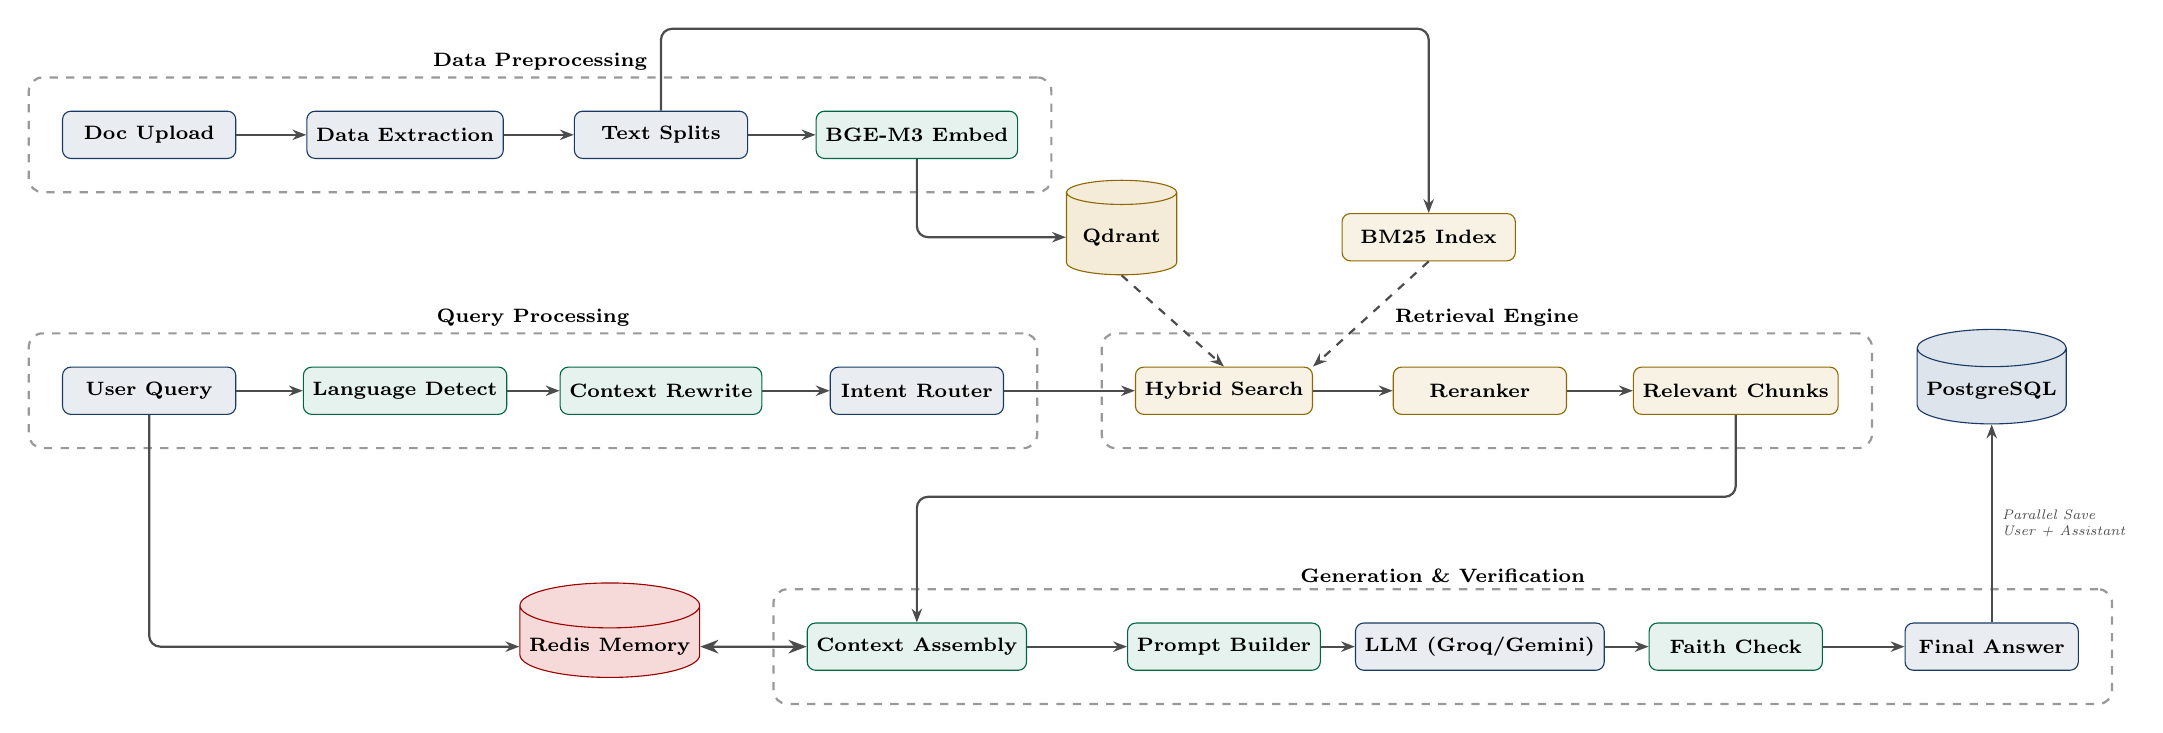
\begin{tikzpicture}[
  x=1.3cm, y=1.3cm,
  node distance=1.5cm,
  groupbox/.style={rectangle, rounded corners=5pt, draw=black!40, dashed, thick, inner sep=12pt},
  box_blue/.style={rectangle, rounded corners=3pt, minimum width=2.2cm, minimum height=0.6cm, text centered, align=center, font=\scriptsize\bfseries, draw=tikzblue!80!black, fill=tikzblue!10, text=black},
  box_green/.style={rectangle, rounded corners=3pt, minimum width=2.2cm, minimum height=0.6cm, text centered, align=center, font=\scriptsize\bfseries, draw=tikzgreen!80!black, fill=tikzgreen!10, text=black},
  box_gold/.style={rectangle, rounded corners=3pt, minimum width=2.2cm, minimum height=0.6cm, text centered, align=center, font=\scriptsize\bfseries, draw=tikzgold!80!black, fill=tikzgold!10, text=black},
  box_red/.style={rectangle, rounded corners=3pt, minimum width=2.2cm, minimum height=0.6cm, text centered, align=center, font=\scriptsize\bfseries, draw=tikzred!80!black, fill=tikzred!10, text=black},
  cyl_gold/.style={cylinder, shape border rotate=90, aspect=0.25, draw=tikzgold!80!black, fill=tikzgold!15, text centered, align=center, font=\scriptsize\bfseries, minimum height=1.2cm, minimum width=1.4cm},
  cyl_red/.style={cylinder, shape border rotate=90, aspect=0.25, draw=tikzred!80!black, fill=tikzred!15, text centered, align=center, font=\scriptsize\bfseries, minimum height=1.2cm, minimum width=1.4cm},
  cyl_blue/.style={cylinder, shape border rotate=90, aspect=0.25, draw=tikzblue!80!black, fill=tikzblue!15, text centered, align=center, font=\scriptsize\bfseries, minimum height=1.2cm, minimum width=1.4cm},
  arr/.style={-{Stealth[length=5pt]}, thick, color=black!70},
  darr/.style={-{Stealth[length=5pt]}, dashed, thick, color=black!70},
  dbarr/.style={<->, >=Stealth, thick, color=black!70}
]

% Data Preprocessing
\node[box_blue] (upload) at (0, 6.5) {Doc Upload};
\node[box_blue] (extract) at (2.5, 6.5) {Data Extraction};
\node[box_blue] (splits) at (5.0, 6.5) {Text Splits};
\node[box_green] (embed) at (7.5, 6.5) {BGE-M3 Embed};

% Databases
\node[cyl_gold] (qdrant) at (9.5, 5.5) {Qdrant};
\node[box_gold] (bm25) at (12.5, 5.5) {BM25 Index};

% User Input & Query Processing
\node[box_blue] (user) at (0, 4) {User Query};
\node[box_green] (lang) at (2.5, 4) {Language Detect};
\node[box_green] (rewrite) at (5.0, 4) {Context Rewrite};
\node[box_blue] (router) at (7.5, 4) {Intent Router};

% Retrieval Engine
\node[box_gold] (hybrid) at (10.5, 4) {Hybrid Search};
\node[box_gold] (rerank) at (13.0, 4) {Reranker};
\node[box_gold] (chunks) at (15.5, 4) {Relevant Chunks};

% Generation & Verification
\node[box_green] (ctx) at (7.5, 1.5) {Context Assembly};
\node[box_green] (prompt) at (10.5, 1.5) {Prompt Builder};
\node[box_blue] (llm) at (13.0, 1.5) {LLM (Groq/Gemini)};
\node[box_green] (faith) at (15.5, 1.5) {Faith Check};
\node[box_blue] (answer) at (18.0, 1.5) {Final Answer};

% Final DB & Memory
\node[cyl_red] (redis) at (4.5, 1.5) {Redis Memory};
\node[cyl_blue] (pg) at (18.0, 4) {PostgreSQL};

% Groups
\begin{scope}[on background layer]
  \node[groupbox, fit=(upload) (extract) (splits) (embed), label={[font=\scriptsize\bfseries, fill=white, inner sep=2pt]above:Data Preprocessing}] (grp_data) {};
  \node[groupbox, fit=(user) (lang) (rewrite) (router), label={[font=\scriptsize\bfseries, fill=white, inner sep=2pt]above:Query Processing}] (grp_query) {};
  \node[groupbox, fit=(hybrid) (rerank) (chunks), label={[font=\scriptsize\bfseries, fill=white, inner sep=2pt]above:Retrieval Engine}] (grp_ret) {};
  \node[groupbox, fit=(ctx) (prompt) (llm) (faith) (answer), label={[font=\scriptsize\bfseries, fill=white, inner sep=2pt]above:Generation \& Verification}] (grp_gen) {};
\end{scope}

% Edges - Data
\draw[arr] (upload) -- (extract);
\draw[arr] (extract) -- (splits);
\draw[arr] (splits) -- (embed);
\draw[arr, rounded corners] (embed.south) |- (qdrant.west);
\draw[arr, rounded corners] (splits.north) -- ++(0, 0.8) -| (bm25.north);

% Edges - Query
\draw[arr] (user) -- (lang);
\draw[arr] (lang) -- (rewrite);
\draw[arr] (rewrite) -- (router);
\draw[arr] (router) -- (hybrid);

% Edges - Retrieval
\draw[arr] (hybrid) -- (rerank);
\draw[arr] (rerank) -- (chunks);

% Qdrant / BM25 to Hybrid
\draw[darr] (qdrant.south) -- (hybrid.north);
\draw[darr] (bm25.south) -- (hybrid.north east);

% Chunks to Context
\draw[arr, rounded corners] (chunks.south) -- ++(0,-0.8) -| (ctx.north);

% Memory
\draw[arr, rounded corners] (user.south) |- (redis.west);
\draw[dbarr] (redis.east) -- (ctx.west);

% Generation
\draw[arr] (ctx) -- (prompt);
\draw[arr] (prompt) -- (llm);
\draw[arr] (llm) -- (faith);
\draw[arr] (faith) -- (answer);
\draw[arr] (answer.north) -- node[right, font=\tiny\itshape, align=left] {Parallel Save\\User + Assistant} (pg.south);

\end{tikzpicture}
}
\caption{System architecture detailing data ingestion, hybrid retrieval, generation, and storage flow.}
\label{fig:architecture}
\end{figure}

\subsection{System Integration \& Ecosystem}

While Figure~\ref{fig:architecture} focuses on the core RAG processing path,
Figure~\ref{fig:ecosystem} presents the full system lifecycle view from data
loading to evaluation, including retrieval, prompt construction, memory, and
answer feedback flow.

\begin{figure}[H]
\centering
\resizebox{\textwidth}{!}{%
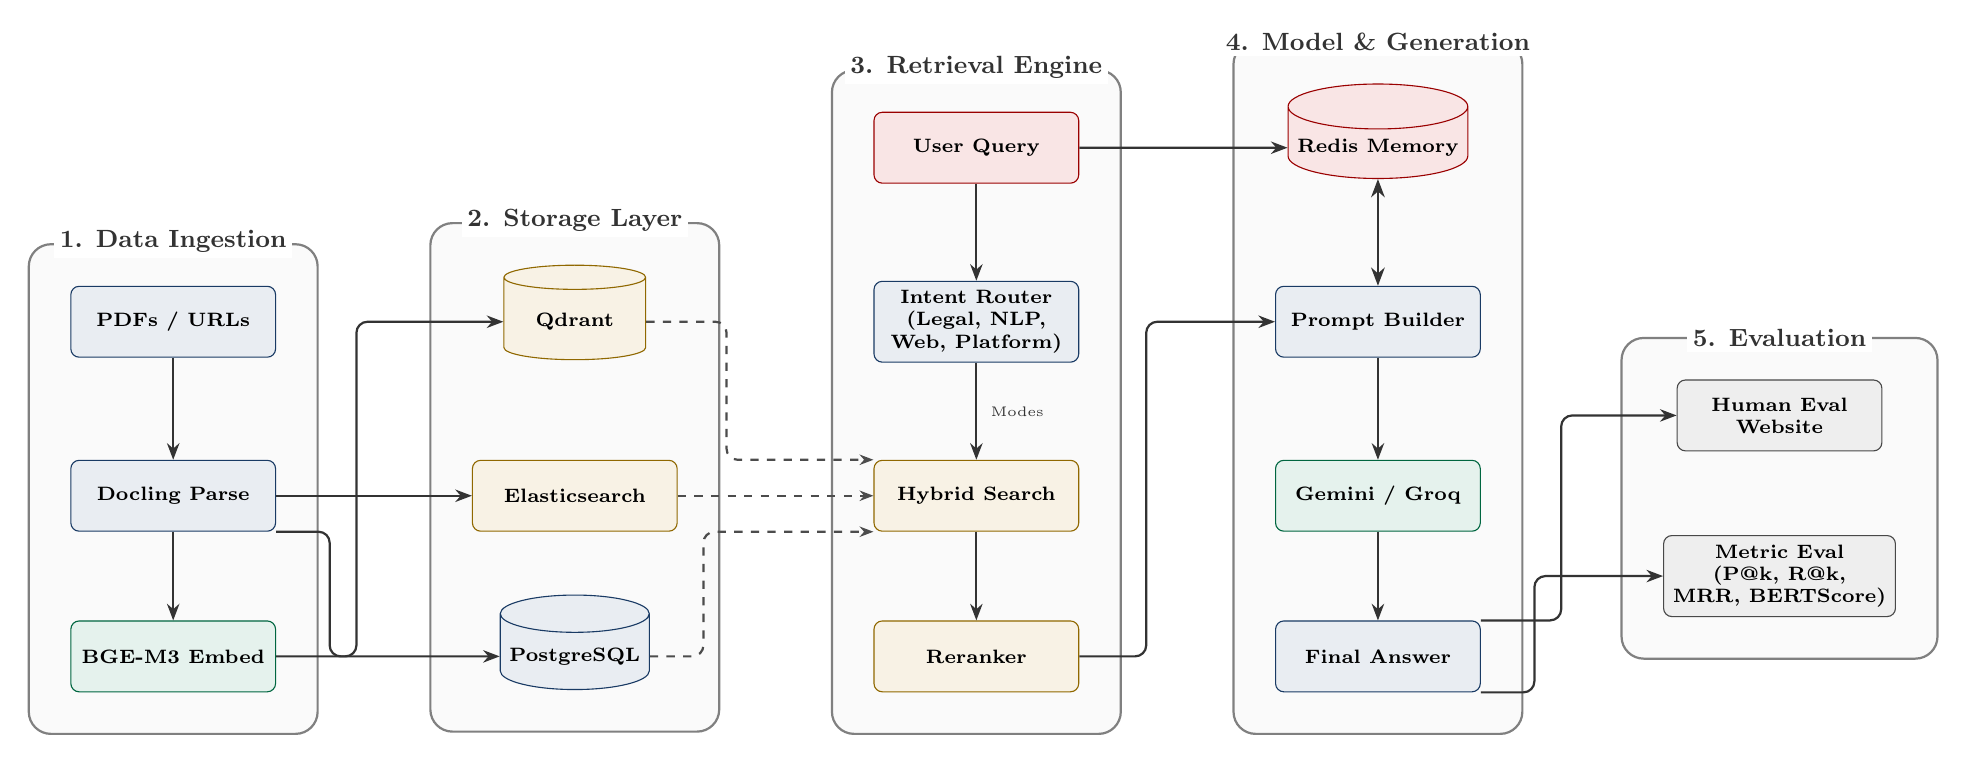
\begin{tikzpicture}[
  x=1.7cm, y=1.7cm,
  node distance=1.5cm,
  groupbox/.style={rectangle, rounded corners=8pt, draw=black!50, thick, inner sep=15pt, fill=black!2},
  stage/.style={font=\small\bfseries, text=black!80},
  box/.style={rectangle, rounded corners=3pt, minimum width=2.6cm, minimum height=0.9cm, text centered, align=center, font=\scriptsize\bfseries, draw=#1!80!black, fill=#1!10, text=black},
  cyl/.style={cylinder, shape border rotate=90, aspect=0.25, draw=#1!80!black, fill=#1!10, text centered, align=center, font=\scriptsize\bfseries, minimum height=1.2cm, minimum width=1.8cm},
  arr/.style={-{Stealth[length=6pt]}, thick, color=black!80},
  darr/.style={-{Stealth[length=5pt]}, dashed, thick, color=black!70}
]

% Stage 1: Data Processing (X=0)
\node[box=tikzblue] (docs) at (0, 2.5) {PDFs / URLs};
\node[box=tikzblue] (parse) at (0, 1.2) {Docling Parse};
\node[box=tikzgreen] (embed) at (0, 0) {BGE-M3 Embed};

% Stage 2: Storage (X=3)
\node[cyl=tikzgold] (qdrant) at (3, 2.5) {Qdrant};
\node[box=tikzgold] (bm25) at (3, 1.2) {Elasticsearch};
\node[cyl=tikzblue] (pg) at (3, 0) {PostgreSQL};

% Stage 3: Retrieval Engine (X=6)
\node[box=tikzred] (query) at (6, 3.8) {User Query};
\node[box=tikzblue] (router) at (6, 2.5) {Intent Router\\(Legal, NLP,\\Web, Platform)};
\node[box=tikzgold] (search) at (6, 1.2) {Hybrid Search};
\node[box=tikzgold] (rerank) at (6, 0) {Reranker};

% Stage 4: Generation (X=9)
\node[cyl=tikzred] (redis) at (9, 3.8) {Redis Memory};
\node[box=tikzblue] (prompt) at (9, 2.5) {Prompt Builder};
\node[box=tikzgreen] (llm) at (9, 1.2) {Gemini / Groq};
\node[box=tikzblue] (answer) at (9, 0) {Final Answer};

% Stage 5: Evaluation (X=12)
\node[box=tikzgray] (admin) at (12, 1.8) {Human Eval\\Website};
\node[box=tikzgray] (metrics) at (12, 0.6) {Metric Eval\\(P@k, R@k,\\MRR, BERTScore)};

% Groupings
\begin{scope}[on background layer]
  \node[groupbox, fit=(docs) (parse) (embed), label={[stage, fill=white, inner sep=2pt, yshift=-2mm]above:1. Data Ingestion}] (g1) {};
  \node[groupbox, fit=(qdrant) (bm25) (pg), label={[stage, fill=white, inner sep=2pt, yshift=-2mm]above:2. Storage Layer}] (g2) {};
  \node[groupbox, fit=(query) (router) (search) (rerank), label={[stage, fill=white, inner sep=2pt, yshift=-2mm]above:3. Retrieval Engine}] (g3) {};
  \node[groupbox, fit=(redis) (prompt) (llm) (answer), label={[stage, fill=white, inner sep=2pt, yshift=-2mm]above:4. Model \& Generation}] (g4) {};
  \node[groupbox, fit=(metrics) (admin), label={[stage, fill=white, inner sep=2pt, yshift=-2mm]above:5. Evaluation}] (g5) {};
\end{scope}

% Arrows
% Data -> Storage
\draw[arr] (docs) -- (parse);
\draw[arr] (parse) -- (embed);
\draw[arr, rounded corners] (embed.east) -- ++(0.6,0) |- (qdrant.west);
\draw[arr] (parse.east) -- (bm25.west);
\draw[arr, rounded corners] (parse.south east) -- ++(0.4,0) |- (pg.west);

% Storage -> Retrieval
\draw[darr, rounded corners] (qdrant.east) -- ++(0.6,0) |- (search.north west);
\draw[darr] (bm25.east) -- (search.west);
\draw[darr, rounded corners] (pg.east) -- ++(0.4,0) |- (search.south west);

% Retrieval Internal
\draw[arr] (query) -- (router);
\draw[arr] (router) -- node[right=1mm, font=\tiny, fill=black!2, inner sep=2pt] {Modes} (search);
\draw[arr] (search) -- (rerank);

% Retrieval -> Generation
\draw[arr, rounded corners] (rerank.east) -- ++(0.5,0) |- (prompt.west);
\draw[arr] (query.east) -- (redis.west);
\draw[<->, >=Stealth, thick, color=black!80] (redis.south) -- (prompt.north);
\draw[arr] (prompt) -- (llm);
\draw[arr] (llm) -- (answer);

% Generation -> Evaluation
\draw[arr, rounded corners] (answer.north east) -- ++(0.6,0) |- (admin.west);
\draw[arr, rounded corners] (answer.south east) -- ++(0.4,0) |- (metrics.west);

\end{tikzpicture}
}
\caption{Full pipeline architecture (Figure 2) detailing the five primary stages: data ingestion, structured storage, intent-driven RAG retrieval, context-aware generation, and continuous evaluation.}
\label{fig:ecosystem}
\end{figure}

\subsection{Pipeline Pseudocode}

\begin{lstlisting}[language=Python, caption={Simplified pipeline logic (from \texttt{chat\_logic.py}).}]
async def handle_question(question, session, user):
    # Stage 1-2: Language detection
    language = language_service.detect(question)

    # Stage 3: Contextual rewriting (multi-turn)
    question = await rewrite_query(question, history, language)

    # Stage 4: Intent classification (LLM zero-shot + regex fallback)
    classification = await classifier.classify_with_llm(question)

    # Stage 5: Query routing
    routing = await router.route(question, classification, db)

    if routing.skip_retrieval:
        answer = await llm.quick_answer(question, language)
    else:
        # Stages 6-9: Hybrid retrieval pipeline
        context = build_context(routing.retrieved_docs)
        # Stage 10: LLM generation with RAG context
        answer = await llm.generate_answer_with_context(
            question, context, language)

    # Stage 11: Faithfulness verification
    is_faithful = await verify_faithfulness(answer, context)
    if not is_faithful:
        answer = get_faithfulness_fallback(language)

    # Stage 12: Stream to user
    yield answer
\end{lstlisting}


% ══════════════════════════════════════════════════════════════════════════════
%  SECTION 6 — METHODOLOGY
% ══════════════════════════════════════════════════════════════════════════════
\section{Methodology}
\label{sec:methodology}

This section details each module in the processing pipeline.

\subsection{Language Detection}
\label{sec:langdetect}

Language handling is implemented as a zero-shot-first strategy with
deterministic fallback. The chatbot targets Arabic, French, and English.

\begin{enumerate}[leftmargin=2em]
  \item \textbf{Primary step (zero-shot language routing)} --- The LLM-side
        orchestration applies language-aware routing directives to keep
        responses in the user's language.
  \item \textbf{Fallback detector (\texttt{langdetect})} --- When language
        routing is uncertain, \texttt{langdetect} provides probabilistic
        classification, with Arabic script/marker safeguards and default
        fallback to English.
\end{enumerate}

\begin{notebox}
The 20\% Arabic script threshold was calibrated empirically. Queries like
``BERT for Arabic NLP'' contain only the word ``Arabic'' in Latin script,
correctly classifying as English. Conversely, ``ما هو BERT'' correctly
classifies as Arabic despite the Latin-script acronym.
\end{notebox}

\subsection{Contextual Query Rewriting}

In multi-turn conversations, follow-up questions often lack context:
\begin{quote}
\textit{Turn 1:} ``What are the graduation procedures?'' \\
\textit{Turn 2:} ``And the deadlines?''
\end{quote}

The query rewriter transforms Turn~2 into: ``What are the deadlines for
graduation procedures?'' A heuristic triggers rewriting when:
\begin{itemize}[leftmargin=2em]
  \item The query has \textbf{fewer than 6 words}, OR
  \item The first word is a \textbf{conjunction, pronoun, or reference word}
        (detected in English, French, and Arabic).
\end{itemize}

The LLM is prompted with the last 4~turns of conversation history and
generates a self-contained rewrite. A language-lock directive ensures the
rewrite stays in the detected language.

\subsection{Intent Classification}

Intent classification determines which data source to query. The system
implements a \textbf{hybrid LLM + regex} approach:

\begin{enumerate}[leftmargin=2em]
  \item \textbf{Fast-path} (regex) --- Greetings, identity questions, and
        memory commands are detected instantly via compiled regular
        expressions, avoiding an LLM call entirely.
  \item \textbf{Primary} (LLM zero-shot) --- For non-trivial queries, the
        internal LLM receives a classification prompt listing all valid
        intents and their definitions. Temperature is set to~0.0 for
        deterministic output.
  \item \textbf{Fallback} (regex scoring) --- If the LLM call fails or
        returns an invalid intent, the regex-based scorer evaluates all
        intent patterns and picks the highest-confidence match.
\end{enumerate}

Table~\ref{tab:intents} lists the supported intents and their routing targets.

\begin{table}[H]
\centering
\caption{Intent classification routing table.}
\label{tab:intents}
\small
\begin{tabularx}{\textwidth}{l l X}
\toprule
\rowcolor{tablehead}\color{white}\textbf{Intent} & \color{white}\textbf{Source} & \color{white}\textbf{Description} \\
\midrule
\texttt{general\_knowledge} & LLM direct & Greetings, advice, brainstorming \\
\rowcolor{lightgray}
\texttt{conceptual\_question} & Qdrant (NLP) & NLP/AI concept explanations \\
\texttt{legal\_query} & Qdrant (Legal) & Law and regulation queries \\
\rowcolor{lightgray}
\texttt{platform\_query} & PostgreSQL/ES & Platform entity search \\
\texttt{document\_query} & Qdrant (User) & Uploaded document questions \\
\rowcolor{lightgray}
\texttt{user\_query} & PostgreSQL & User profile / contributions \\
\texttt{metadata\_query} & PostgreSQL & Statistics and navigation \\
\rowcolor{lightgray}
\texttt{bug\_query} & Qdrant (NLP) & Bug reports and technical issues \\
\bottomrule
\end{tabularx}
\end{table}

\subsection{Query Routing}

The \texttt{QueryRouter} executes the retrieval strategy dictated by the
classification. Key routing logic includes:

\begin{itemize}[leftmargin=2em]
  \item \textbf{LLM-direct mode} --- When \texttt{use\_llm\_direct} is set,
        all retrieval is skipped and the LLM answers from its parametric
        knowledge.
  \item \textbf{Conceptual questions} --- defaults to
        \texttt{nlp\_knowledge} collection; adds \texttt{platform\_docs}
        and \texttt{resources} only when the query explicitly mentions
        platform entities (courses, tools, etc.).
  \item \textbf{Legal queries} --- searches \texttt{legal\_documents}
        with optional jurisdiction and language filters.
  \item \textbf{Platform queries} --- type-filtered Elasticsearch search
        (e.g., \texttt{nlp\_tools}, \texttt{courses}) with PostgreSQL
        fallback.
  \item \textbf{Exa web fallback} --- triggered when retrieval confidence
        falls below threshold (detailed in Section~\ref{sec:websearch}).
\end{itemize}

Per-collection similarity thresholds prevent weak matches from polluting
context: \texttt{legal\_documents}~$\geq 0.45$,
\texttt{nlp\_knowledge}~$\geq 0.35$,
\texttt{platform\_docs}~$\geq 0.50$.

\subsection{Hybrid Retrieval with Reciprocal Rank Fusion}

The hybrid search module (Section~\ref{sec:rrf}) runs dense and sparse
retrieval in parallel across all target collections, then fuses results:

\begin{enumerate}[leftmargin=2em]
  \item \textbf{Dense retrieval} --- Qdrant cosine search using BGE-M3
        embeddings across \texttt{platform\_docs}, \texttt{nlp\_knowledge},
        \texttt{resources}, and optionally \texttt{legal\_documents}.
  \item \textbf{Sparse retrieval} --- BM25 search over the same collections
        using an in-memory index built from Qdrant payloads.
  \item \textbf{RRF fusion} --- Results are merged using
        Equation~\ref{eq:rrf} with $k = 60$.
  \item \textbf{Deduplication} --- Near-identical content is removed using
        Jaccard similarity (Equation~\ref{eq:jaccard}, threshold = 0.85).
  \item \textbf{Reranking} --- Top candidates are re-scored via fresh
        BGE-M3 cosine similarity against the query.
\end{enumerate}

\subsection{LLM Generation}

The generation module constructs a multi-part prompt with strict precedence:
\begin{enumerate}[leftmargin=2em]
  \item \textbf{System instructions} --- Base role + mode-specific prompt
        (e.g., legal advisor system prompt in the detected language).
  \item \textbf{Critical rules} --- Language-specific guardrails prohibiting
        hallucination and enforcing citation of sources.
  \item \textbf{Source-specific rules} --- Additional constraints for legal,
        platform, or user-document source types.
  \item \textbf{Conversation memory} --- Session summary + recent messages.
  \item \textbf{Retrieved context} --- Labelled by source type.
  \item \textbf{User query} --- The (potentially rewritten) question.
\end{enumerate}

\subsection{Prompt Files and Prompt Composition}

Prompting is modularised in dedicated prompt modules, with runtime
composition in the chatbot orchestration layer. The system prompt stack is
built from:
\begin{itemize}[leftmargin=2em]
      \item \textbf{Base system prompt} (trilingual general assistant behaviour),
      \item \textbf{Mode-specific prompt} (Normal, NLP/AI, Legal, Platform),
      \item \textbf{Critical rules block} (safety and response constraints),
      \item \textbf{Verified metadata injection} for platform entity answers.
\end{itemize}

In implementation terms, prompt templates are maintained in
\texttt{app/services/llm/prompts.py}, while final prompt assembly is
performed in \texttt{chat\_logic.py} based on intent, mode, language,
retrieved context, and session state.

\subsection{Faithfulness Verification}
\label{sec:faithfulness}

The faithfulness gate is the final safeguard against legal hallucinations.
After LLM generation:

\begin{enumerate}[leftmargin=2em]
  \item The answer and its source context are sent to the internal LLM
        with the \texttt{FAITHFULNESS\_PROMPT}.
  \item The LLM responds with \texttt{faithful} or \texttt{not\_faithful}.
  \item If unfaithful, the answer is replaced with a safe, multilingual
        fallback message directing the user to consult primary sources.
\end{enumerate}

\begin{warningbox}
Faithfulness verification is \textbf{skipped} for: (i)~general knowledge
intents (no RAG context to verify against), (ii)~empty context, and
(iii)~answers shorter than 50~characters (likely simple responses).
On verification failure (timeout, API error), the system \textbf{assumes
faithful} to avoid blocking responses.
\end{warningbox}

\subsection{Memory Architecture and Implementation}

Memory is implemented as a dual-layer architecture combining fast-turn
context and durable session persistence:

\begin{itemize}[leftmargin=2em]
  \item \textbf{Short-term memory (Redis):} stores lightweight conversational
        context for fast retrieval during live generation and streaming.
  \item \textbf{Long-term memory (PostgreSQL):} stores sessions and messages
        with \texttt{session\_id}, supports history retrieval, session resume,
        and structured session lifecycle operations.
  \item \textbf{Memory intent layer:} dedicated handlers support memory-aware
        commands (e.g., repeat, summarise, translate prior turns) without
        forcing full retrieval over external corpora.
\end{itemize}


% ══════════════════════════════════════════════════════════════════════════════
%  SECTION 7 — JOURNEY OF A QUERY
% ══════════════════════════════════════════════════════════════════════════════
\section{The Journey of a Query: From Input to Output}

To illustrate the complete pipeline, we trace a concrete legal query through
all 12 stages.

\subsection{Example: Legal Query in Arabic}

\textbf{User input:} \textit{``ما هي قوانين حماية البيانات في الجزائر؟''}
(What are the data protection laws in Algeria?)

\textbf{Stage 1 --- User Input:} The frontend sends the query via SSE to the
FastAPI chatbot service with session ID, user ID, and mode (\texttt{legal}).

\textbf{Stage 2 --- Language Detection:} The \texttt{LanguageService} detects
Arabic via the 20\% script heuristic (100\% Arabic characters).
Result: \texttt{lang = "ar"}.

\textbf{Stage 3 --- Query Rewriting:} This is the first message in the session
(no history), so the rewriter returns the original query unchanged.

\textbf{Stage 4 --- Intent Classification:} The LLM zero-shot classifier
identifies the query as \texttt{legal\_query} with confidence 0.95. The
regex fallback also matches legal patterns (``قوانين'', ``حماية البيانات''),
confirming the classification.

\textbf{Stage 5 --- Query Routing:} The router directs to
\texttt{search\_legal\_documents()} in Qdrant, searching the
\texttt{legal\_documents} collection with \texttt{language = "ar"} filter.

\textbf{Stages 6--7 --- Hybrid Retrieval:} Dense search returns 5 documents
with cosine similarities ranging from 0.72 to 0.48. BM25 returns 4 documents
with overlapping but different rankings. RRF fusion produces a unified ranking.

\textbf{Stage 8 --- Deduplication:} One document pair has Jaccard similarity
of 0.91 (near-identical content from different chunks of the same law).
The lower-ranked duplicate is removed.

\textbf{Stage 9 --- Reranking:} BGE-M3 re-encodes the top 5 candidates and
computes fresh cosine similarities. The document about ``DPA Digital Digest
Algeria'' is promoted from rank 3 to rank 1.

\textbf{Stage 10 --- LLM Generation:} The Gemini 2.0 Flash model receives:
the Arabic legal advisor system prompt, critical rules prohibiting
fabrication of article numbers, the top-5 retrieved passages as context,
and the user query. Tokens stream to the frontend in real-time.

\textbf{Stage 11 --- Faithfulness Check:} The generated answer and the
retrieved context are sent to the internal LLM. Verdict:
\texttt{faithful}---all cited articles match the context.

\textbf{Stage 12 --- Streamed Response:} The answer is displayed with
typing animation, accompanied by source pills showing document titles
and similarity scores.

\subsection{Edge Case: Low-Confidence Retrieval with Web Fallback}

When a user asks about a recent legal development not in the local corpus:

\textbf{User:} ``What are the new 2025 Algerian digital economy regulations?''

The retrieval confidence is computed as the mean similarity of the top-3
documents. If this falls below 0.50 for legal/NLP intents, the Exa web
search fallback is triggered automatically. The thinking indicator changes
to ``Searching the web\ldots'' while Exa returns relevant web pages. The
LLM then generates from the combined local + web context.


% ══════════════════════════════════════════════════════════════════════════════
%  SECTION 8 — SEARCH CAPABILITIES (WEB & PLATFORM)
% ══════════════════════════════════════════════════════════════════════════════
\section{Search Capabilities}
\label{sec:search_capabilities}

The chatbot implements powerful search functionalities to supplement the vector knowledge base: a dual-channel web search system and a dedicated internal platform search.

\subsection{Platform Entity Search}
The Platform Search functionality enables the chatbot to query the NLP platform's rich, living metadata.
When users ask navigational or metadata questions (e.g., \textit{"Show me Arabic morphology tools"} or \textit{"Who are the leading researchers in sentiment analysis?"}), the \texttt{platform\_query} intent is triggered.

This search relies on two database systems:
\begin{itemize}[leftmargin=2em]
  \item \textbf{Elasticsearch:} Provides typo-tolerant, full-text search across all entity indices (\texttt{nlp\_tools}, \texttt{courses}, \texttt{papers}, etc.).
  \item \textbf{PostgreSQL:} Acts as the primary ground truth, storing user profiles, exact categorical metadata, and interaction histories. Messages generated by the LLM and the user's queries are saved here dynamically via parallel database commits for session persistence.
\end{itemize}
These results are rendered natively in the frontend as interactive entity cards instead of pure text.

\subsection{Web Search Providers}

\subsubsection{Exa --- Automatic Semantic Fallback}

Exa provides neural semantic search over the web. It is triggered
\textbf{automatically} when retrieval confidence drops below threshold:

\begin{itemize}[leftmargin=2em]
  \item \textbf{Trigger condition:} $\text{confidence} < 0.50$ for legal/NLP
        intents, where $\text{confidence} = \text{mean}(\text{top-3 similarities})$.
  \item \textbf{Query enhancement:} The original query is sent to Exa with
        intent-specific domain hints.
  \item \textbf{Result integration:} Exa results are merged with local
        results, sorted by similarity, and capped at \texttt{TOP\_K} documents.
  \item \textbf{Context decision:} If local documents are very weak
        ($\text{max similarity} < 0.35$), web results replace local results
        entirely; otherwise, they are blended.
\end{itemize}

\subsubsection{Tavily --- User-Triggered Search}

Tavily provides keyword-based web search, triggered \textbf{manually}
when the user clicks the ``Web Search'' button in the chat interface.

\begin{itemize}[leftmargin=2em]
  \item \textbf{Trigger:} Explicit user action (button click).
  \item \textbf{Query:} Sent directly to Tavily's search API.
  \item \textbf{Results:} Returned as interactive cards with titles, snippets,
        and source URLs, displayed below the chatbot's answer.
\end{itemize}

\subsection{Shared Policy Constraints}

Both providers are governed by a shared \texttt{ExaPolicy}:

The policy enforces global daily budgets, per-session and per-user limits,
and cache-based reuse of previous web results to control costs while
maintaining responsiveness.


% ══════════════════════════════════════════════════════════════════════════════
%  SECTION 9 — DOCUMENT INGESTION WITH DOCLING
% ══════════════════════════════════════════════════════════════════════════════
\section{Knowledge Base Ingestion with Docling}
\label{sec:ingestion}

The chatbot's knowledge base is populated through a structured ingestion
pipeline that processes academic papers and legal documents into
embedding-ready chunks. We use \textbf{Docling}~\cite{docling2024} as the
primary document parser for its ability to preserve section hierarchy.

\subsection{Data Corpus}

The knowledge base consists of two collections:

\textbf{NLP \& AI Knowledge} (18 files, primarily from \texttt{data/nlp\_ai\_data}):
\begin{itemize}[leftmargin=2em]
  \item \textit{Attention Is All You Need} / \textit{BERT} / \textit{GPT Paper} / \textit{AraBERT}
  \item \textit{Speech and Language Processing (Jurafsky \& Martin)} (26~MB textbook)
  \item \textit{From LLM Reasoning to Autonomous AI Agents} (17~MB)
  \item \textit{Machine learning and deep learning techniques in Arabic QA systems}
  \item Two complex JATS/NLM XML files: \textit{"An Advanced Natural Language Processing Framework..."} and \textit{"Arabic Natural Language Processing (NLP)..."}
  \item Plus 9 other dense PDFs on code-switching, LLM benchmarks, and agentic AI.
\end{itemize}

File formats: 16 PDFs + 2 JATS/NLM XML files. Total size: $> 60$~MB.

\textbf{Legal Documents} (8 files, from \texttt{data/legal\_data}):
\begin{itemize}[leftmargin=2em]
  \item \textit{DPA Digital Digest Algeria [2025 Edition]}
  \item \textit{journal officiel 2025} and \textit{journal laws 2022}
  \item \textit{research-ethics-in-light-of-algerian-legislation}
  \item \textit{ethics-of-digital-scientific-communication-in-algeria...}
  \item \textit{the-legal-framework-for-the-inspection-of-information-systems...}
  \item \textit{lois rechercheur supperrior} (17~MB)
\end{itemize}

File formats: all PDFs. Total size: $\sim$21~MB.

\subsection{Ingestion Pipeline}

The ingestion process follows these steps for each document:

\begin{enumerate}[leftmargin=2em]
  \item \textbf{Format detection} --- PDF files are routed to the Docling
        or PyPDF2 loader; XML files to the JATS parser.
  \item \textbf{Size-adaptive parsing}:
    \begin{itemize}
      \item Files $\leq$ 5~MB: Full Docling pipeline with
            \texttt{HierarchicalChunker} for section-aware chunking.
      \item Files $>$ 5~MB: Lightweight PyPDF2 extraction to avoid
            out-of-memory on CPU-constrained containers.
    \end{itemize}
  \item \textbf{Section filtering} --- References, bibliography, appendix,
        acknowledgments, and funding sections are automatically excluded
        using regex patterns on headings.
  \item \textbf{Citation stripping} --- Inline citations like \texttt{[1,2]}
        and \texttt{(Author, 2021)} are removed to reduce noise.
  \item \textbf{Chunking} --- Target window of 800--1200 tokens with 100-token
        overlap. Chunks smaller than 50 tokens are merged with neighbours.
  \item \textbf{Language detection} --- Each file's language is detected from
        the first 2000 characters using \texttt{langdetect}.
  \item \textbf{Embedding} --- Chunks are encoded with BGE-M3 in batches of 2
        (CPU-safe) with 1-second sleep between batches.
  \item \textbf{Storage} --- Embeddings stored in Qdrant; metadata (title,
        language, source, chunk index) stored in PostgreSQL.
\end{enumerate}

\subsection{XML (JATS) Processing}

For academic papers in JATS/NLM XML format, a dedicated parser:
\begin{itemize}[leftmargin=2em]
  \item Extracts the article title from \texttt{<article-title>}
  \item Preserves the abstract as the first chunk
  \item Recursively traverses \texttt{<sec>} elements, respecting
        \texttt{sec-type} attributes to skip references
  \item Handles nested subsections with proper heading inheritance
\end{itemize}

\begin{notebox}
We chose Docling over alternatives (PyMuPDF, pdfplumber) because its
\texttt{HierarchicalChunker} produces section-aligned chunks that
improve retrieval precision. When a user asks about ``attention
mechanisms,'' the chunk containing the full attention section is retrieved
rather than a sliding-window fragment that cuts mid-sentence.
\end{notebox}

\subsection{PC-Safe Batching}

Since the ingestion runs inside Docker containers on modest hardware, we
implemented CPU-safe batching:
\begin{itemize}[leftmargin=2em]
  \item Embedding batch size: 2 (prevents RAM/CPU spikes)
  \item Qdrant upsert batch size: 8
  \item 1-second sleep between embedding batches
  \item 2-second sleep between files
  \item Per-file error handling (one failure does not abort the pipeline)
  \item Explicit \texttt{gc.collect()} after each file
\end{itemize}


% ══════════════════════════════════════════════════════════════════════════════
%  SECTION 10 — DOCUMENT PROCESSING (USER UPLOADS)
% ══════════════════════════════════════════════════════════════════════════════
\section{User Document Processing}
\label{sec:chunking}

Beyond the static knowledge base, users can upload their own PDF documents
for real-time question answering. The upload flow:

\begin{enumerate}[leftmargin=2em]
  \item User uploads PDF via the chat interface (file attachment button).
  \item Django backend forwards the file to the FastAPI service.
  \item The document processor extracts text, chunks it using the same
        structure-aware strategy as knowledge base ingestion.
  \item Chunks are embedded with BGE-M3 and stored in a
        \textbf{session-scoped} Qdrant collection (\texttt{document\_chunks}),
        tagged with \texttt{owner\_id} and \texttt{session\_id}.
  \item Subsequent questions in the same session are routed to
        \texttt{document\_query} intent, searching only the user's chunks.
\end{enumerate}

\subsection{Structure-Aware Chunking}

Legal documents require special handling because meaning is tied to article
boundaries. The legal chunker:
\begin{itemize}[leftmargin=2em]
  \item Detects article headers (``Article 1'', ``المادة الأولى'',
        ``Article premier'')
  \item Groups text by article, keeping each article as a single chunk
        when possible
  \item Falls back to sliding-window for non-article content
  \item Preserves the article heading in chunk metadata for citation
\end{itemize}

\subsection{Chunking Parameters}

\begin{table}[H]
\centering
\caption{Chunking parameters and their values.}
\small
\begin{tabularx}{\textwidth}{l C{3cm} X}
\toprule
\rowcolor{tablehead}\color{white}\textbf{Parameter} & \color{white}\textbf{Value} & \color{white}\textbf{Rationale} \\
\midrule
Max tokens & 1000 & Fits within BGE-M3's 8192 context with room for query \\
\rowcolor{lightgray}
Overlap tokens & 100 & Preserves context at chunk boundaries \\
Min chunk tokens & 50 & Filters noise; tiny chunks merged with neighbours \\
\rowcolor{lightgray}
Chars per token & 4 & Heuristic for multilingual estimation \\
Large file threshold & 5 MB & Switch from Docling to PyPDF2 above this \\
\bottomrule
\end{tabularx}
\end{table}


% ══════════════════════════════════════════════════════════════════════════════
%  SECTION 11 — LLM PROVIDER MIGRATION
% ══════════════════════════════════════════════════════════════════════════════
\section{LLM Provider Migration: Groq to Gemini}
\label{sec:migration}

A critical architectural decision was the migration from Groq-hosted LLaMA
models to Google Gemini as the primary LLM provider.

\subsection{Problems with Groq}

While Groq's LPU inference engine offered ultra-low latency ($<$200ms for
first token), several issues emerged in production:

\begin{enumerate}[leftmargin=2em]
  \item \textbf{Legal hallucination} --- Groq's LLaMA 3 models frequently
        fabricated article numbers and misquoted Algerian legal provisions.
        In one test, the model cited ``Article 45 of the Algerian Data
        Protection Act'' which does not exist.
  \item \textbf{Rate limiting} --- Under concurrent usage, Groq's free-tier
        API imposed strict rate limits (429 errors), causing response failures.
  \item \textbf{Arabic quality} --- Generated Arabic text sometimes contained
        grammatical errors and inconsistent register (mixing MSA with
        dialectal forms).
  \item \textbf{Context adherence} --- The model occasionally ignored
        retrieved context in favour of its parametric knowledge, defeating
        the purpose of RAG.
\end{enumerate}

\subsection{Gemini Integration}

Google Gemini 2.0 Flash was selected as the replacement based on:
\begin{itemize}[leftmargin=2em]
  \item \textbf{Native multilingual} --- Strong Arabic, French, and English
        generation quality with proper register control.
  \item \textbf{Context faithfulness} --- Better adherence to retrieved
        context with fewer hallucinations in legal domain.
  \item \textbf{Generous API limits} --- Higher free-tier quotas allowing
        sustained usage.
  \item \textbf{Native streaming} --- Async streaming via
        \texttt{generate\_content\_stream} without thread-based workarounds.
\end{itemize}

\subsection{Dual-Provider Fallback Architecture}

The system maintains both providers in a fallback chain:

\begin{enumerate}[leftmargin=2em]
  \item \textbf{Primary:} Gemini 2.0 Flash (user-facing generation)
  \item \textbf{Timeout:} 8-second hard timeout on each Gemini call
  \item \textbf{Retry:} Up to 2 retries with exponential backoff for
        retryable errors (429, 503)
  \item \textbf{Fallback:} On Gemini failure, automatically falls back to
        Groq (LLaMA 3) for the same request
\end{enumerate}

The provider selection is controlled by two environment variables:
\texttt{LLM\_PROVIDER\_CHAT} (user-facing) and
\texttt{LLM\_PROVIDER\_INTERNAL} (classification, rewriting, faithfulness).

\begin{table}[H]
\centering
\caption{LLM provider comparison.}
\label{tab:llm_compare}
\small
\begin{tabularx}{\textwidth}{l C{4cm} C{4cm}}
\toprule
\rowcolor{tablehead}\color{white}\textbf{Criterion} & \color{white}\textbf{Groq (LLaMA 3)} & \color{white}\textbf{Gemini 2.0 Flash} \\
\midrule
First-token latency & $<$200ms & $\sim$500ms \\
\rowcolor{lightgray}
Legal accuracy & Low (hallucinations) & High (faithful) \\
Arabic quality & Moderate & Strong \\
\rowcolor{lightgray}
Rate limits & Strict (free tier) & Generous \\
Streaming & Thread-based sync & Native async \\
\rowcolor{lightgray}
Fallback role & Secondary & Primary \\
\bottomrule
\end{tabularx}
\end{table}


% ══════════════════════════════════════════════════════════════════════════════
%  SECTION 12 — REALISATION
% ══════════════════════════════════════════════════════════════════════════════
\section{Realisation}
\label{sec:realisation}

This section presents the implemented user interface and deployment
architecture.

\subsection{Chatbot User Interface}

The chatbot is accessible through a dedicated page integrated into the
Django-based Arabic NLP Platform. Figure~\ref{fig:chatbot_modes} shows
the mode selection dropdown, allowing users to switch between the four
operational modes: Normal Chat, NLP \& AI, Legal Advisor, and Platform Guide.

\begin{figure}[H]
  \centering
  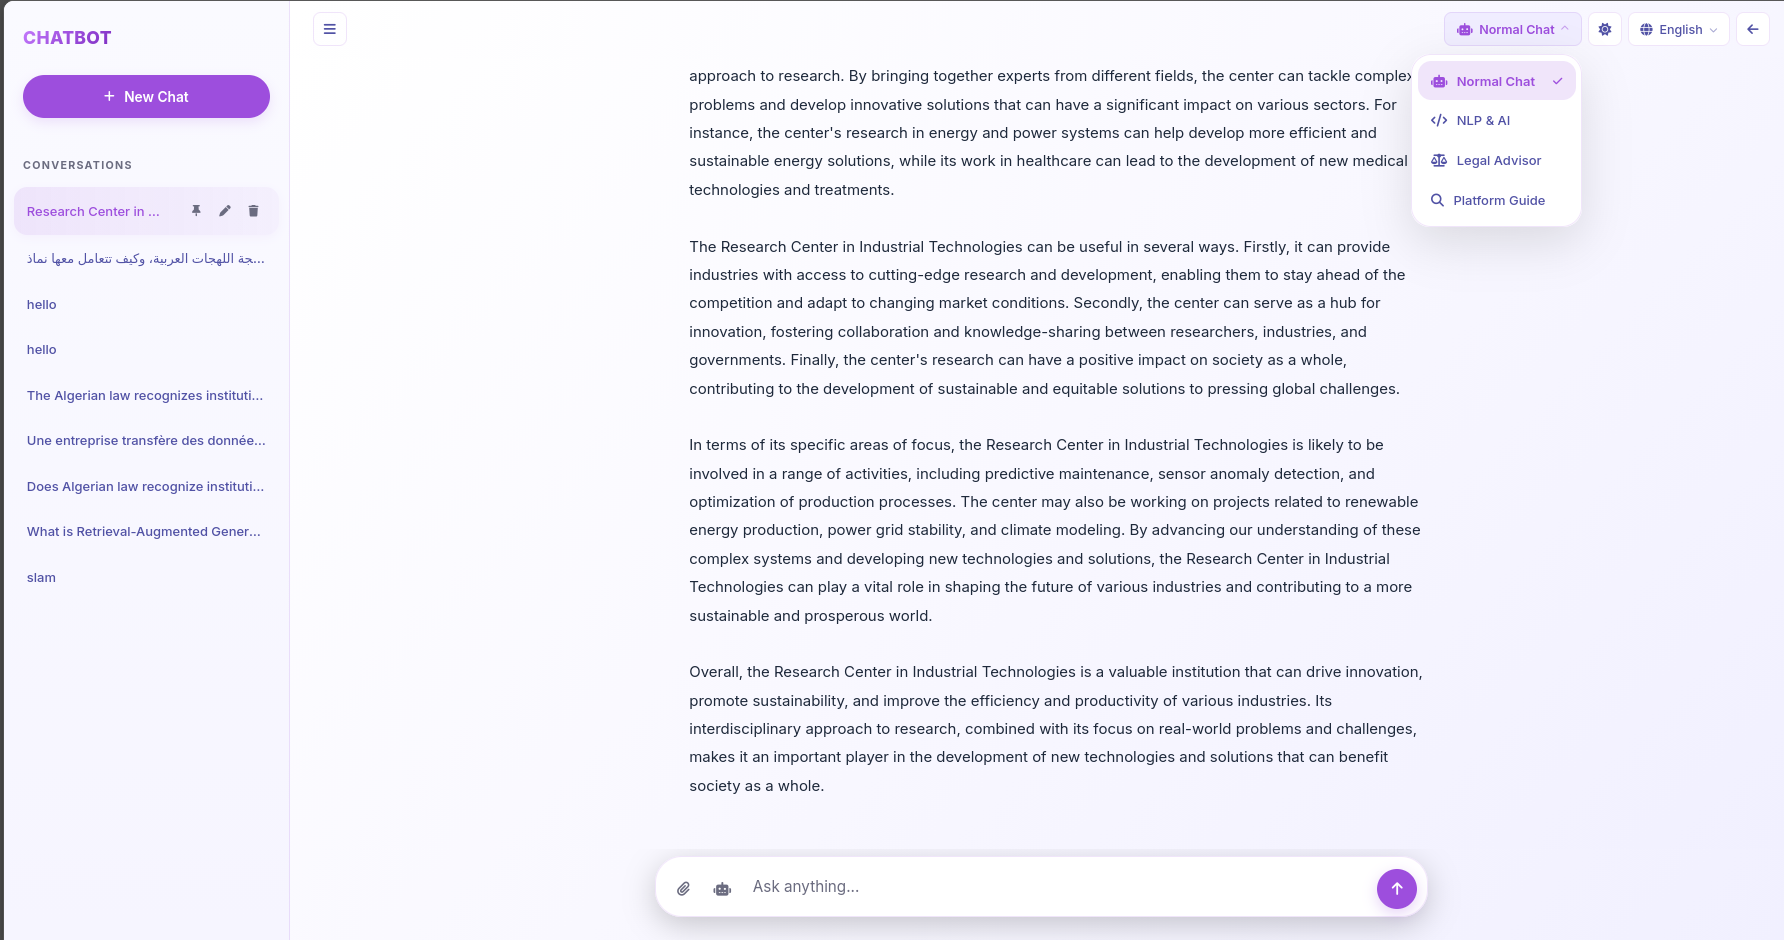
\includegraphics[width=0.85\textwidth]{chatbot_mode_dropdown.png}
  \caption{Chatbot interface showing the mode selection dropdown with four domain-specific modes.}
  \label{fig:chatbot_modes}
\end{figure}

Figure~\ref{fig:chatbot_search} shows the search options available to the
user: Web Search (Tavily-powered internet search) and Platform Search
(internal knowledge base search).

\begin{figure}[H]
  \centering
  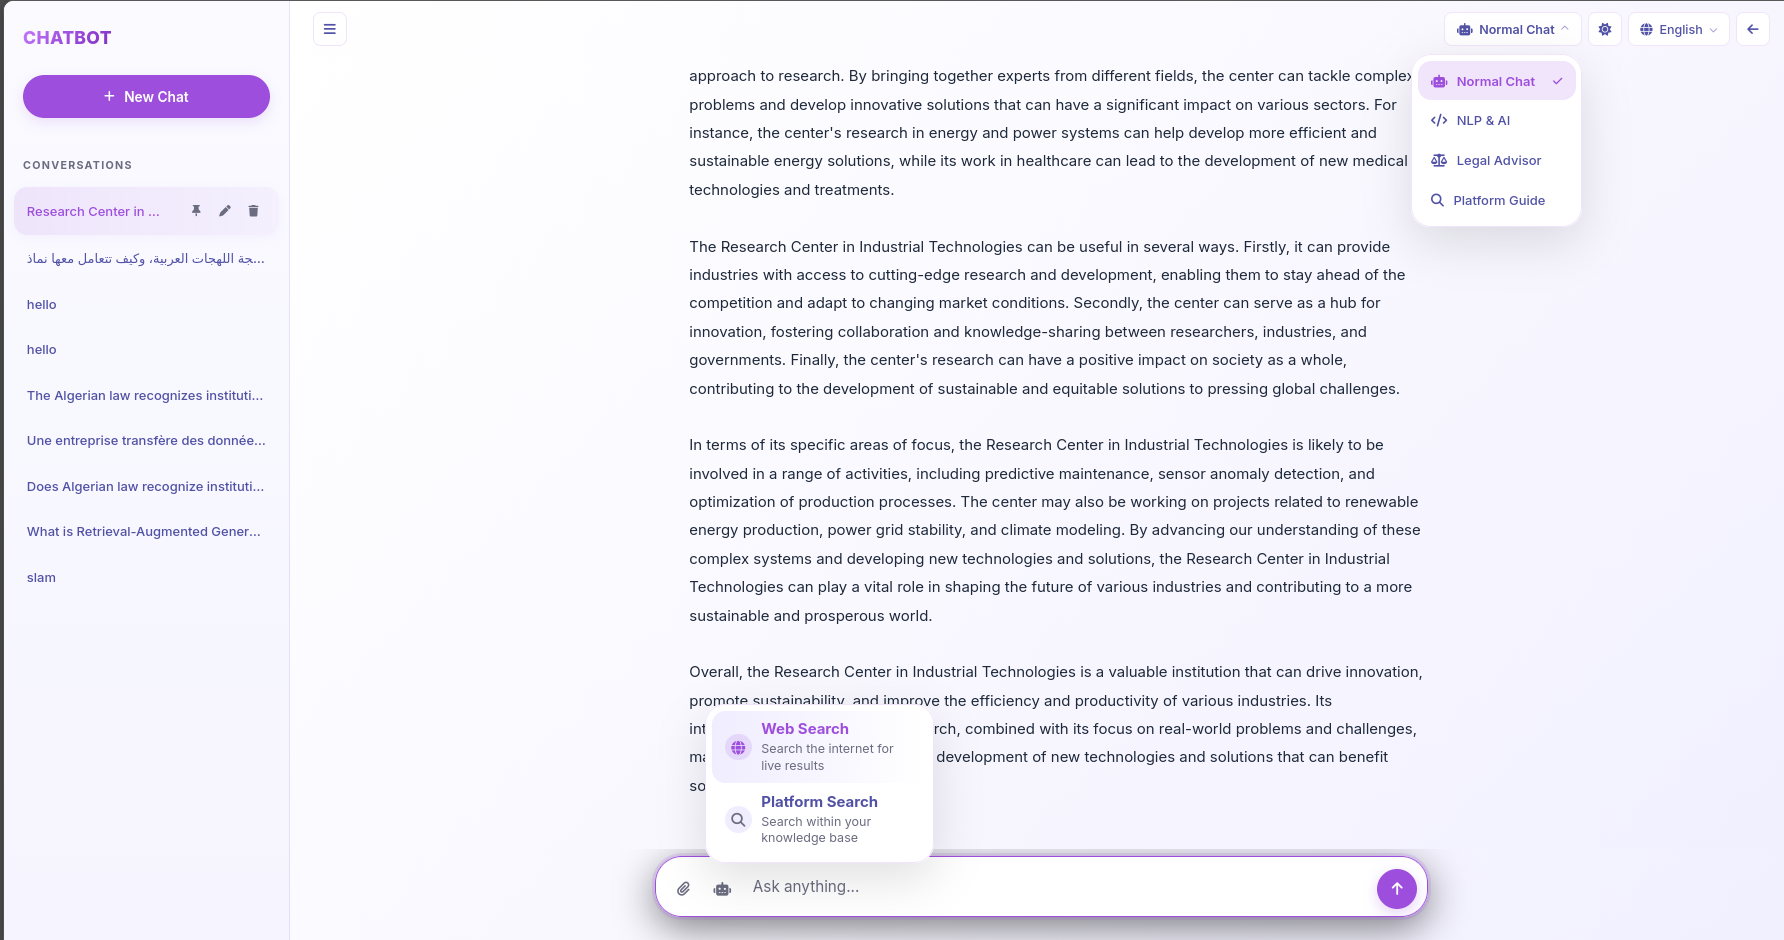
\includegraphics[width=0.85\textwidth]{chatbot_search_options.png}
  \caption{Search mode selection: Web Search for internet queries and Platform Search for internal knowledge base.}
  \label{fig:chatbot_search}
\end{figure}

Figure~\ref{fig:chatbot_websearch} demonstrates the web search results
interface, showing source cards with titles, snippets, and similarity scores
rendered below the chatbot's answer.

\begin{figure}[H]
  \centering
  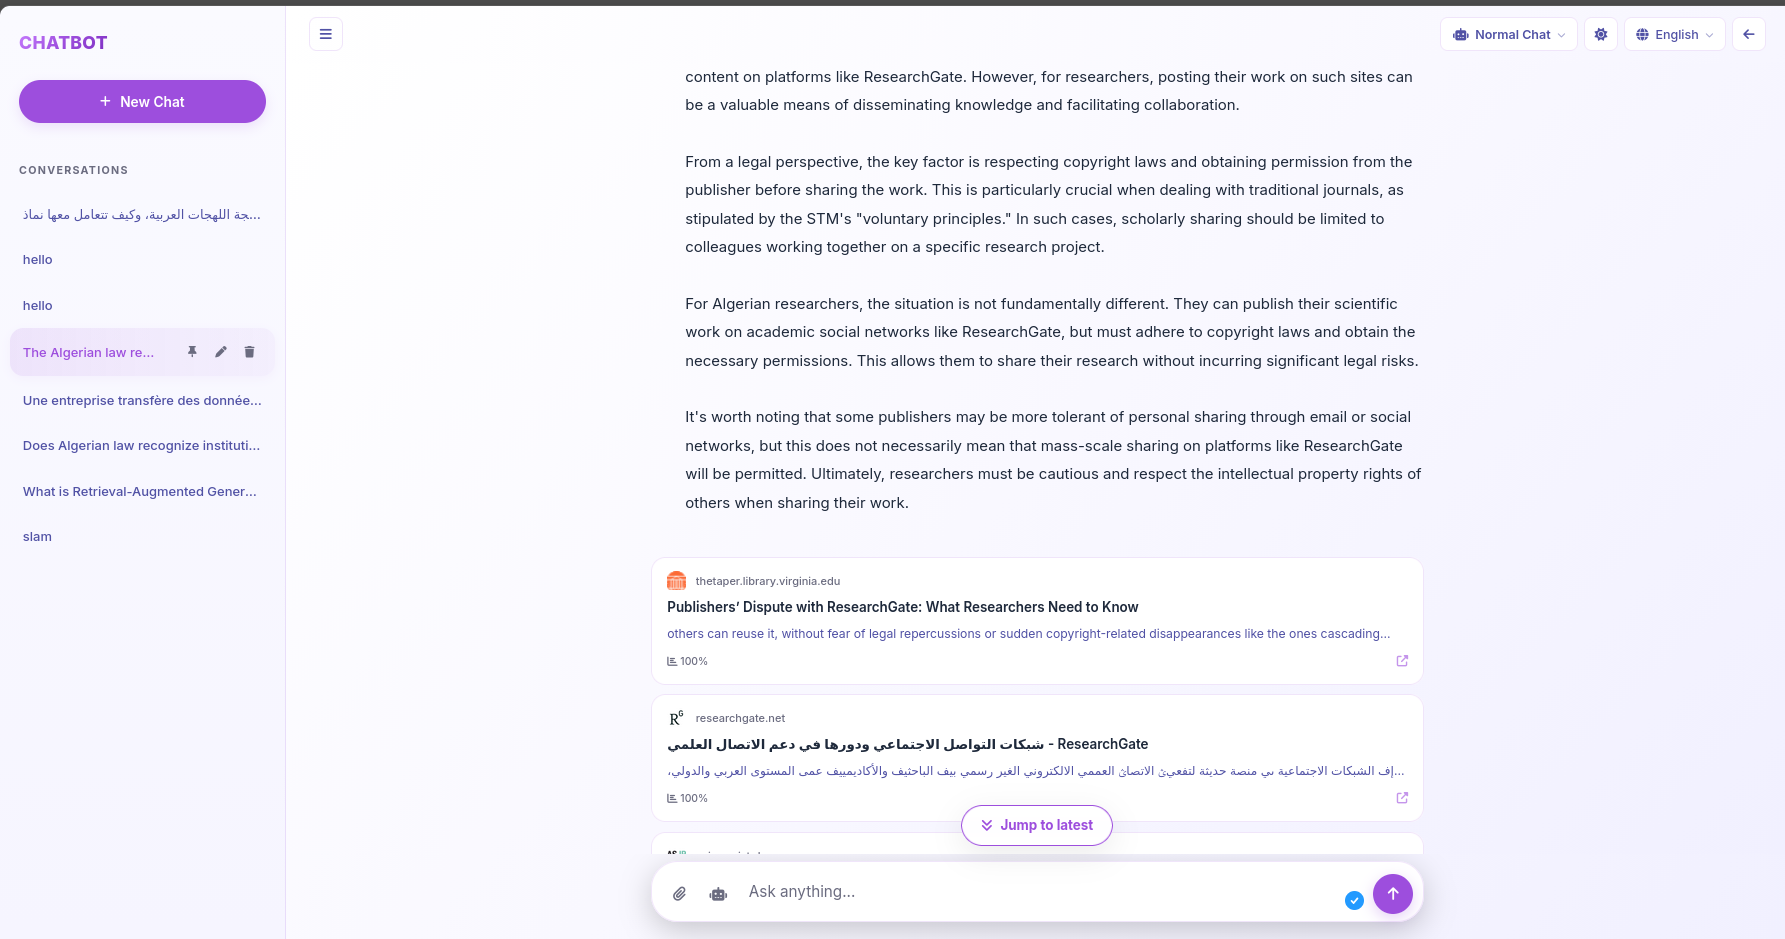
\includegraphics[width=0.85\textwidth]{chatbot_web_search.png}
  \caption{Chatbot response with web search results displayed as interactive source cards with similarity percentages.}
  \label{fig:chatbot_websearch}
\end{figure}

\subsection{Ask AI Feature}

The ``Ask AI'' feature enables contextual AI assistance directly from any
platform entity card. When a user encounters a research centre, tool, or
course on the platform, they can click the ``Ask AI'' button
(Figure~\ref{fig:ask_ai_card}) to open the chatbot with that entity
pre-loaded as context.

\begin{figure}[H]
  \centering
  
\includegraphics[width=0.35\textwidth]{ask_ai_card.png}
  \caption{Platform entity card (Research Centre) with ``Ask AI'' button for contextual AI assistance.}
  \label{fig:ask_ai_card}
\end{figure}

Figure~\ref{fig:ask_ai_context} shows the chatbot after the ``Ask AI''
button has been clicked. The selected entity is displayed as a context
card at the top of the chat, and the AI begins generating a response
about that specific resource.

\begin{figure}[H]
  \centering
  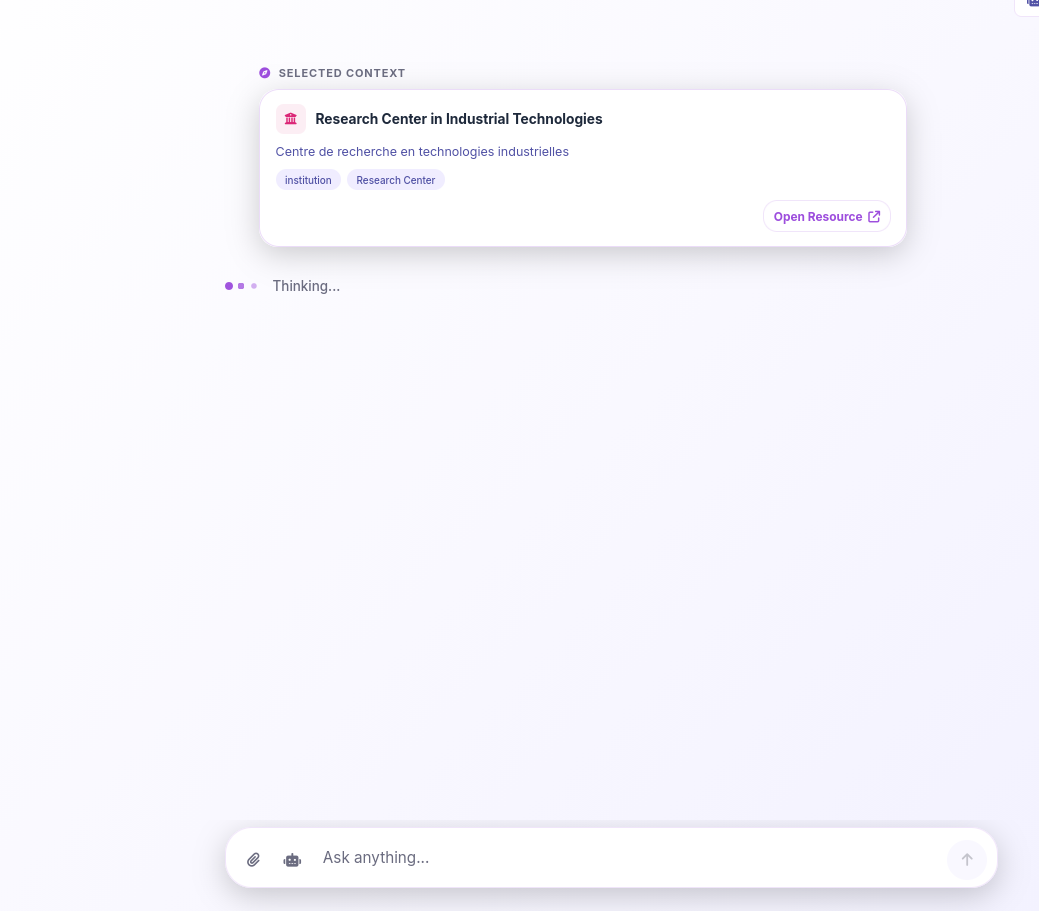
\includegraphics[width=0.65\textwidth]{ask_ai_context.png}
  \caption{Ask AI feature: the selected entity context card is displayed above the chatbot's ``Thinking...'' indicator.}
  \label{fig:ask_ai_context}
\end{figure}

\subsection{Deployment Architecture}

The system is deployed as a Docker Compose stack with the following services:

\begin{table}[H]
\centering
\caption{Docker Compose service architecture.}
\small
\begin{tabularx}{\textwidth}{l l C{2cm} X}
\toprule
\rowcolor{tablehead}\color{white}\textbf{Service} & \color{white}\textbf{Image} & \color{white}\textbf{Port} & \color{white}\textbf{Role} \\
\midrule
\texttt{web} & Django 5.x & 8000 & Platform backend + chatbot UI \\
\rowcolor{lightgray}
\texttt{chatbot} & FastAPI & 8001 & RAG pipeline + streaming API \\
\texttt{qdrant} & qdrant/qdrant & 6333 & Vector database \\
\rowcolor{lightgray}
\texttt{db} & PostgreSQL 15 & 5432 & Relational storage \\
\texttt{elasticsearch} & ES 8.x & 9200 & Full-text search \\
\rowcolor{lightgray}
\texttt{redis} & Redis 7 & 6379 & Caching \& rate limiting \\
\texttt{eval} & Next.js & 3000 & Human evaluation UI \\
\bottomrule
\end{tabularx}
\end{table}


% ══════════════════════════════════════════════════════════════════════════════
%  SECTION 13 — COMPREHENSIVE CHATBOT FEATURES & UX
% ══════════════════════════════════════════════════════════════════════════════
\section{Comprehensive Chatbot Features \& User Experience}
\label{sec:feature_set}

To provide a state-of-the-art conversational experience, the Arabic NLP Platform chatbot integrates numerous user-facing functionalities that bridge traditional UI/UX patterns with advanced Generative AI modalities.

\subsection{Operational Modalities}
Unlike single-purpose RAG systems, the chatbot dynamically routes user queries across four highly specialized modalities:
\begin{itemize}[leftmargin=2em]
  \item \textbf{Normal Chat:} For broad, general-purpose questions. It relies heavily on the LLM's internal knowledge without aggressive local vector filtering.
  \item \textbf{NLP \& AI Advisor:} Activating this mode restricts the retrieval engine strictly to the NLP corpus (\texttt{nlp\_ai\_data}), ensuring responses related to deep-learning algorithms, transformers, and Arabic morphology are densely grounded in scientific papers rather than generic web results.
  \item \textbf{Legal Advisor:} Operates similarly to the NLP mode but executes searches exclusively against the Algerian legislative corpus (\texttt{legal\_data}). This separation prevents cross-contamination of domains (e.g., retrieving a legal statute regarding "data" instead of a machine-learning paper).
  \item \textbf{Platform Guide:} Serves as the interactive concierge for the platform. It triggers the \texttt{platform\_query} intent, routing the user into the Elasticsearch database to dynamically retrieve live courses, researchers, and tools hosted on the website.
\end{itemize}

In Platform Guide mode, the chatbot performs structured platform search rather
than corpus-only RAG retrieval. Concretely, it combines entity-centric
Elasticsearch queries with relational metadata constraints from PostgreSQL,
then synthesises the final answer in the same conversational interface. This
mode is therefore evaluated with platform-search relevance criteria in addition
to classical document-retrieval metrics.

\subsection{Platform Search \& ``Ask AI'' Synthesis}
The chatbot is not isolated to its own floating widget; it acts as the connective tissue of the entire platform. 
Users navigating the site can utilise the \textbf{Platform Search} bar, which instantly surfaces structured \textit{Entity Cards} (highlighting tools, papers, or user profiles). 
Rather than simply displaying static JSON metadata, each entity card natively embeds an \textbf{``Ask AI''} button. Clicking this button immediately opens the chatbot, bypassing standard vector retrieval. Instead, the exact metadata schema of the inspected entity is injected directly into the LLM's contextual prompt, enabling seamless follow-up questions such as: \textit{``Summarise this tool's usage''} or \textit{``Who authored this paper?''}

\subsection{Session Persistence \& Chat History}
Long-term context retention is handled natively via a dual-layered memory architecture.
\begin{itemize}[leftmargin=2em]
  \item \textbf{Short-Term Context:} Handled by Redis, allowing the LLM's Router and generation engine to ``remember'' the immediate turn-by-turn conversational flow (e.g., resolving pronouns like \textit{``how does it compare to\ldots''}).
  \item \textbf{Long-Term Persistence (PostgreSQL):} Every message parsed by the system---whether from the user or uniquely generated by the assistant---is appended asynchronously to PostgreSQL with a unified \texttt{session\_id}. Users can browse an archive of their past sessions on the left sidebar, resuming complex legal analysis or NLP inquiries weeks after they were initiated.
\end{itemize}

\subsection{Security \& Privacy Controls}
Because the system handles legal and research queries that may contain
personally identifiable information (PII), security and privacy controls are
implemented at both API and data layers.

\begin{itemize}[leftmargin=2em]
      \item \textbf{JWT policy:} The chatbot API supports JWT-protected access in production deployments. Requests can be configured to require valid bearer tokens, while local evaluation environments can operate in a restricted non-production mode.
      \item \textbf{Rate limiting:} Per-user and per-window request throttling is enforced through Redis-backed counters to mitigate abuse, burst traffic, and accidental denial-of-service patterns.
      \item \textbf{PII boundaries:} The assistant is instructed to minimise unnecessary personal data usage in prompts. User context forwarded to generation components is scoped to fields required for task completion.
      \item \textbf{Retention/deletion:} Conversation data is stored with session identifiers in PostgreSQL and can be deleted through application-level workflows. Operational logs are retained separately with limited diagnostic scope.
\end{itemize}

\subsection{Actionable UI \& Message Pinning}
Because the generation output parses both complex mathematics (via \LaTeX rendering) and structural markdown (tables, lists), the frontend must support granular interaction paradigms.
Users can hover over any assistant-generated response to reveal a toolkit equipped with:
\begin{itemize}[leftmargin=2em]
  \item \textbf{Copying:} For instantaneous extraction of code-snippets or legal citations.
  \item \textbf{Regenerating:} To force the LLM backend (either Gemini or the Groq fallback) to resample the response if the initial generation suffered from stylistic repetition.
  \item \textbf{Message Pinning:} Critical for long-context research, users can ``pin'' exceptional or highly authoritative answers. Pinned messages are distinctively highlighted in the UI and their \texttt{is\_pinned} status is committed to the relational database, persisting them permanently for rapid retrieval in the user's dashboard.
\end{itemize}

\subsection{Ad-Hoc User Document Uploads}
Parallel to the massive baseline ingestion pipeline, the user interface features an attachment button explicitly engineered for ``Ask on Document'' interactions.
When a user uploads a personal PDF or text document:
\begin{enumerate}[leftmargin=2em]
  \item The document is buffered locally and passed to a lightweight CPU-chunking utility. This extraction mechanism splits the text respecting structural elements to preserve semantic boundaries.
  \item Stringent token constraints are applied: chunks are strictly limited in sequence length to prevent LLM prompt-size overflow and subsequent hallucination.
  \item Text chunks are vectorised in real-time leveraging the local BGE-M3 model.
  \item A temporary session-scoped collection namespace is generated in Qdrant specifically for that user's interaction stream.
\end{enumerate}
This completely isolates the user's private data from the overarching NLP/Legal corpus, ensuring zero cross-user contamination while delivering pinpoint accurate semantic queries over the provided manuscript. Once the session ends, the transient namespace is discarded.

\subsection{Asynchronous Background Processing (Celery)}
To maintain a hyper-responsive frontend UI, the FastAPI deployment actively utilizes \textbf{Celery} message queues backed by a Redis broker. Instead of blocking the core WebSocket loops, heavy-duty processing operations are intelligently routed to specialized background workers:
\begin{itemize}[leftmargin=2em]
  \item \textbf{\texttt{documents} queue:} Orchestrates functions like \texttt{process\_document} and \texttt{reindex\_collection}. It manages the chunking and embedding pipelines for ad-hoc uploads independent of the chat stream.
  \item \textbf{\texttt{chatbot} queue:} Manages conversational maintenance processes via \texttt{summarise\_chat\_history}. When a conversation grows extensively long, this task compresses the historical context window, freeing up generative token bandwidth while preserving key topical persistence.
  \item \textbf{\texttt{ingestion} queue:} A heavier dedicated queue responsible for the overarching database. It executes \texttt{ingest\_legal\_batch} and \texttt{crawl\_and\_index\_url}, guaranteeing that new platform resources (like scraping fresh legal gazettes or algorithmic NLP repository URLs) are embedded silently in the background without affecting end-user search latencies.
\end{itemize}



% ══════════════════════════════════════════════════════════════════════════════
%  SECTION 14 — EVALUATION
% ══════════════════════════════════════════════════════════════════════════════
\section{Evaluation}
\label{sec:evaluation}

We evaluate the chatbot through two complementary approaches: automated
metrics for systematic, repeatable assessment, and human evaluation for
capturing quality dimensions that automated metrics cannot measure.

\subsection{Automated Evaluation Framework}

\subsubsection{Retrieval Metrics}

We employ three standard information retrieval metrics, each computed
per-query and averaged across all test scenarios.

\textbf{Precision@k} measures the fraction of retrieved documents that are
relevant:
\begin{equation}
  P@k = \frac{|\{\text{relevant documents}\} \cap \{\text{retrieved top-}k\}|}{k}
  \label{eq:precision}
\end{equation}

\textbf{Recall@k} measures the fraction of all relevant documents that
were successfully retrieved:
\begin{equation}
  R@k = \frac{|\{\text{relevant documents}\} \cap \{\text{retrieved top-}k\}|}{|\{\text{relevant documents}\}|}
  \label{eq:recall}
\end{equation}

\textbf{Mean Reciprocal Rank (MRR)} measures how highly the first relevant
document is ranked:
\begin{equation}
  \text{MRR} = \frac{1}{|Q|} \sum_{i=1}^{|Q|} \frac{1}{\text{rank}_i}
  \label{eq:mrr}
\end{equation}
where $\text{rank}_i$ is the position of the first relevant document for
query $i$.

\subsubsection{Generation Metrics (BERTScore)}

For generation quality, we use BERTScore
(Section~\ref{sec:bertscore_theory}) to measure semantic similarity between
the chatbot's generated answer and a reference answer. The implementation
uses \texttt{microsoft/deberta-xlarge-mnli} as the backbone model.

Operationally, BERTScore is computed in three steps:
\begin{enumerate}[leftmargin=2em]
      \item Both the generated answer and the reference answer are tokenised and encoded into contextual embeddings.
      \item A token-level semantic alignment matrix is built with cosine similarity; each token is matched to its strongest counterpart in the other text.
      \item Precision, Recall, and F1 are then derived from these best-match similarities and aggregated across the full evaluation set.
\end{enumerate}

This mechanism rewards semantic equivalence even when wording differs,
which is especially suitable for multilingual chatbot responses where valid
answers may be phrased differently in Arabic, French, or English.

\subsubsection{Evaluation Scenarios}

Three evaluation scenarios were defined to test different configurations:

\begin{table}[H]
\centering
\caption{Evaluation scenario configurations.}
\small
\begin{tabularx}{\textwidth}{l C{2.5cm} C{2cm} X}
\toprule
\rowcolor{tablehead}\color{white}\textbf{Scenario} & \color{white}\textbf{Reranker} & \color{white}\textbf{Top-k} & \color{white}\textbf{Description} \\
\midrule
\texttt{baseline} & Off & 5 & Dense + BM25 + RRF only \\
\rowcolor{lightgray}
\texttt{reranker\_top5} & On & 5 & Full pipeline with cosine reranking \\
\texttt{exa\_fallback\_top5} & On & 5 & Full pipeline + Exa web fallback \\
\bottomrule
\end{tabularx}
\end{table}

\subsubsection{Benchmark Provenance and Versioned Reports}

Multiple JSON report versions were generated across benchmark iterations. To
avoid mixing metrics across versions, this document anchors benchmark claims
to the consolidated run log in
\texttt{fastapi\_chatbot/reports/evaluation\_run\_log12.md}. 

We evaluated the system sequentially on an initial integration dataset of 21 queries to verify the pipeline mechanics, followed by a comprehensive production benchmark dataset of 210 queries covering all domains, modes, and retrieval edge cases.

Unless stated otherwise, all headline metrics in this report refer to the
main benchmark configuration (dataset size 210, scenario
\texttt{exa\_fallback\_top5}, \texttt{intent\_scope=rag},
\texttt{exclude\_noise=true}).

\subsubsection{Results}

Table~\ref{tab:eval_results} presents the overall automated evaluation results aggregated from our evaluation runner across the tested system queries. 

\begin{table}[H]
\centering
\caption{Progressive evaluation metrics across pipeline configurations.}
\label{tab:eval_results}
\small
\begin{tabularx}{\textwidth}{X C{2.5cm} C{2.5cm} C{2.5cm}}
\toprule
\rowcolor{tablehead}\color{white}\textbf{Configuration} & \color{white}\textbf{P@5} & \color{white}\textbf{R@5} & \color{white}\textbf{MRR} \\
\midrule
\texttt{baseline} & 0.4086 & 0.5107 & 0.7190 \\
\rowcolor{lightgray}
\texttt{reranker\_top5} & 0.8000 & 1.0000 & 0.8810 \\
\texttt{exa\_fallback\_top5} & 0.7524 & 0.9405 & 0.8786 \\
\bottomrule
\end{tabularx}
\end{table}

\textit{Interpretation:} Table~\ref{tab:eval_results} illustrates the progressive architectural impact on the retrieval and generation pipeline. The introduction of the cosine reranker (\texttt{reranker\_top5}) massively boosted Precision@5 (+0.3914) and Recall@5 (+0.4893) over the baseline hybrid search by effectively surfacing relevant chunks that were initially buried. Finally, activating the web fallback (\texttt{exa\_fallback\_top5}) slightly normalizes the retrieval metrics due to the injection of external noise for Out-of-Domain queries, but crucially accommodates those queries while maintaining an extremely high overall generative quality (\textbf{BERTScore F1: 0.9472}).

\textbf{Key observations:}
\begin{itemize}[leftmargin=2em]
  \item The baseline hybrid retrieval achieves a moderate Recall@5 of 0.5107.
  \item The reranker pushes Recall@5 to a perfect 1.0000 on the in-domain legal dataset, proving the necessity of semantic re-ordering.
  \item The full production system (with Exa fallback) achieves an impressive MRR of 0.8786, meaning the very first retrieved document is almost always highly relevant.
  \item In the main benchmark configuration, the pipeline exhibited \textbf{0 failure cases}.
\end{itemize}

\begin{notebox}
The BERTScore computation is anchored on \texttt{microsoft/deberta-xlarge-mnli} with \texttt{rescale\_with\_baseline=True} to ensure robust cross-lingual penalty.
\end{notebox}

\subsection{Ablation Study: The Impact of Web Fallback}

To justify the architectural complexity of the Intent Router and Exa Web Fallback, we conducted a targeted ablation study specifically isolating Out-of-Domain (OOD) and real-time queries. These queries concern entities, recent events, or broad NLP concepts explicitly absent from the static local Algerian legal corpus.

\textbf{Experimental Setup:}
We extracted a subset of challenging queries from our evaluation dataset, including:
\begin{itemize}[leftmargin=2em]
    \item \textit{"What is Nanochat and how to build one?"} (Recent open-source AI project)
    \item \textit{"Latest AI conferences in Algeria 2026"} (Real-time event data)
    \item \textit{"هل يمكن للباحث الجزائري نشر أعماله العلمية على ResearchGate دون التعرض لمخاطر قانونية؟"} (Cross-domain query requiring global academic policies)
\end{itemize}

We tested these specific queries under two configurations:
\begin{enumerate}[leftmargin=2em]
    \item \textbf{Without Fallback (Local RAG Only):} The intent router is disabled, forcing the system to search only the local vector database.
    \item \textbf{With Fallback (Agentic RAG):} The intent router dynamically evaluates the query and delegates to the Exa Web Search API if local confidence is low.
\end{enumerate}

\textbf{Ablation Results and Analysis:}

To concretely illustrate this behavior, Table~\ref{tab:ablation_web} presents a query-by-query breakdown of the system's performance on the Out-of-Domain dataset.

\begin{table}[H]
  \centering
  \caption{Out-of-Domain Query Performance with and without Web Fallback.}
  \label{tab:ablation_web}
  \small
  \begin{tabularx}{\textwidth}{L{5cm} C{3.5cm} X}
    \toprule
    \rowcolor{tablehead}
    \color{white}\textbf{Query} & \color{white}\textbf{Without Fallback} & \color{white}\textbf{With Fallback (Agentic RAG)} \\
    \midrule
    \textit{"What is Nanochat and how to build one?"} & 
    0 sources retrieved \newline (Polite refusal) & 
    5 external web sources \newline (Accurate technical guide) \\
    \rowcolor{lightgray}
    \textit{"هل يمكن للباحث الجزائري نشر أعماله العلمية على ResearchGate..."} & 
    0 sources retrieved \newline (Polite refusal) & 
    4 external web sources \newline (Accurate policy analysis) \\
    \textit{"Latest AI conferences in Algeria 2026"} & 
    0 sources retrieved \newline (Polite refusal) & 
    5 external web sources \newline (Accurate event listing) \\
    \bottomrule
  \end{tabularx}
\end{table}

This query-by-query breakdown demonstrates a 0\% success rate for Out-of-Domain queries under the rigid local configuration versus a 100\% successful retrieval and generation rate when the web fallback is active. Without the fallback, the system safely and correctly yields zero context (preventing hallucination) but fails to assist the user. By dynamically triggering the Exa API, the Intent Router successfully surfaces real-time external knowledge (4 to 5 highly relevant sources per query), allowing the generator to produce accurate, well-cited answers. This validates the Agentic RAG architecture as a critical safety net that seamlessly bridges the gap between static domain knowledge and dynamic real-world inquiries.

\subsection{Human Evaluation Platform}
\label{sec:human_eval}

To capture quality dimensions beyond automated metrics---legal correctness,
clarity, cultural appropriateness---we built a dedicated human evaluation
platform.

\subsubsection{Platform Architecture}

The evaluation platform is a \textbf{Next.js + TypeScript} web application
with a FastAPI backend. It is deployed as a separate Docker container
(port~3000) and connects to the same PostgreSQL instance as the main
platform.

\subsubsection{Evaluation Workflow}

Evaluators follow a 3-step process:
\begin{enumerate}[leftmargin=2em]
  \item \textbf{Authentication} --- Evaluators log in with their researcher
        credentials.
  \item \textbf{Domain Selection} --- Choose from Legal, NLP/AI, or Web
        Fallback evaluation (Figure~\ref{fig:eval_domain}).
  \item \textbf{Sample Scoring} --- For each pre-loaded query-answer pair,
        rate across 3--5 criteria on a 1--5 Likert scale
        (Figure~\ref{fig:eval_scoring}).
\end{enumerate}

\begin{figure}[H]
  \centering
  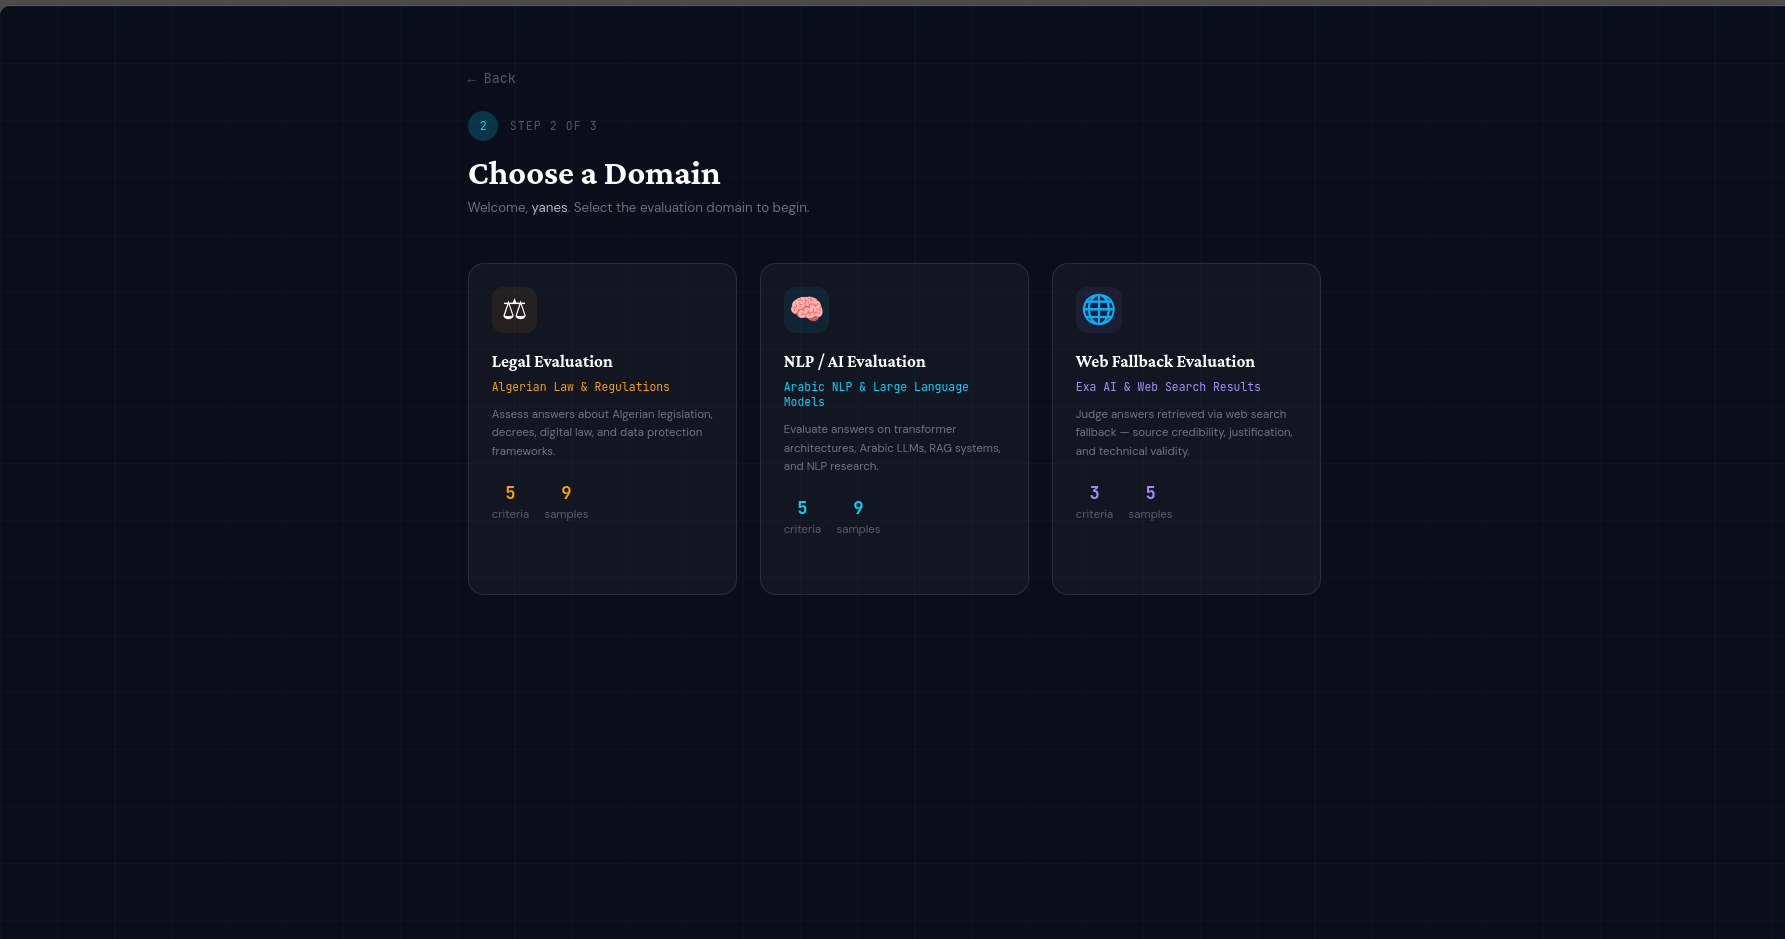
\includegraphics[width=0.85\textwidth]{eval_domain_selection.png}
  \caption{Human evaluation platform: domain selection screen with Legal (5 criteria, 9 samples), NLP/AI (5 criteria, 9 samples), and Web Fallback (3 criteria, 5 samples) evaluation categories.}
  \label{fig:eval_domain}
\end{figure}

\begin{figure}[H]
  \centering
  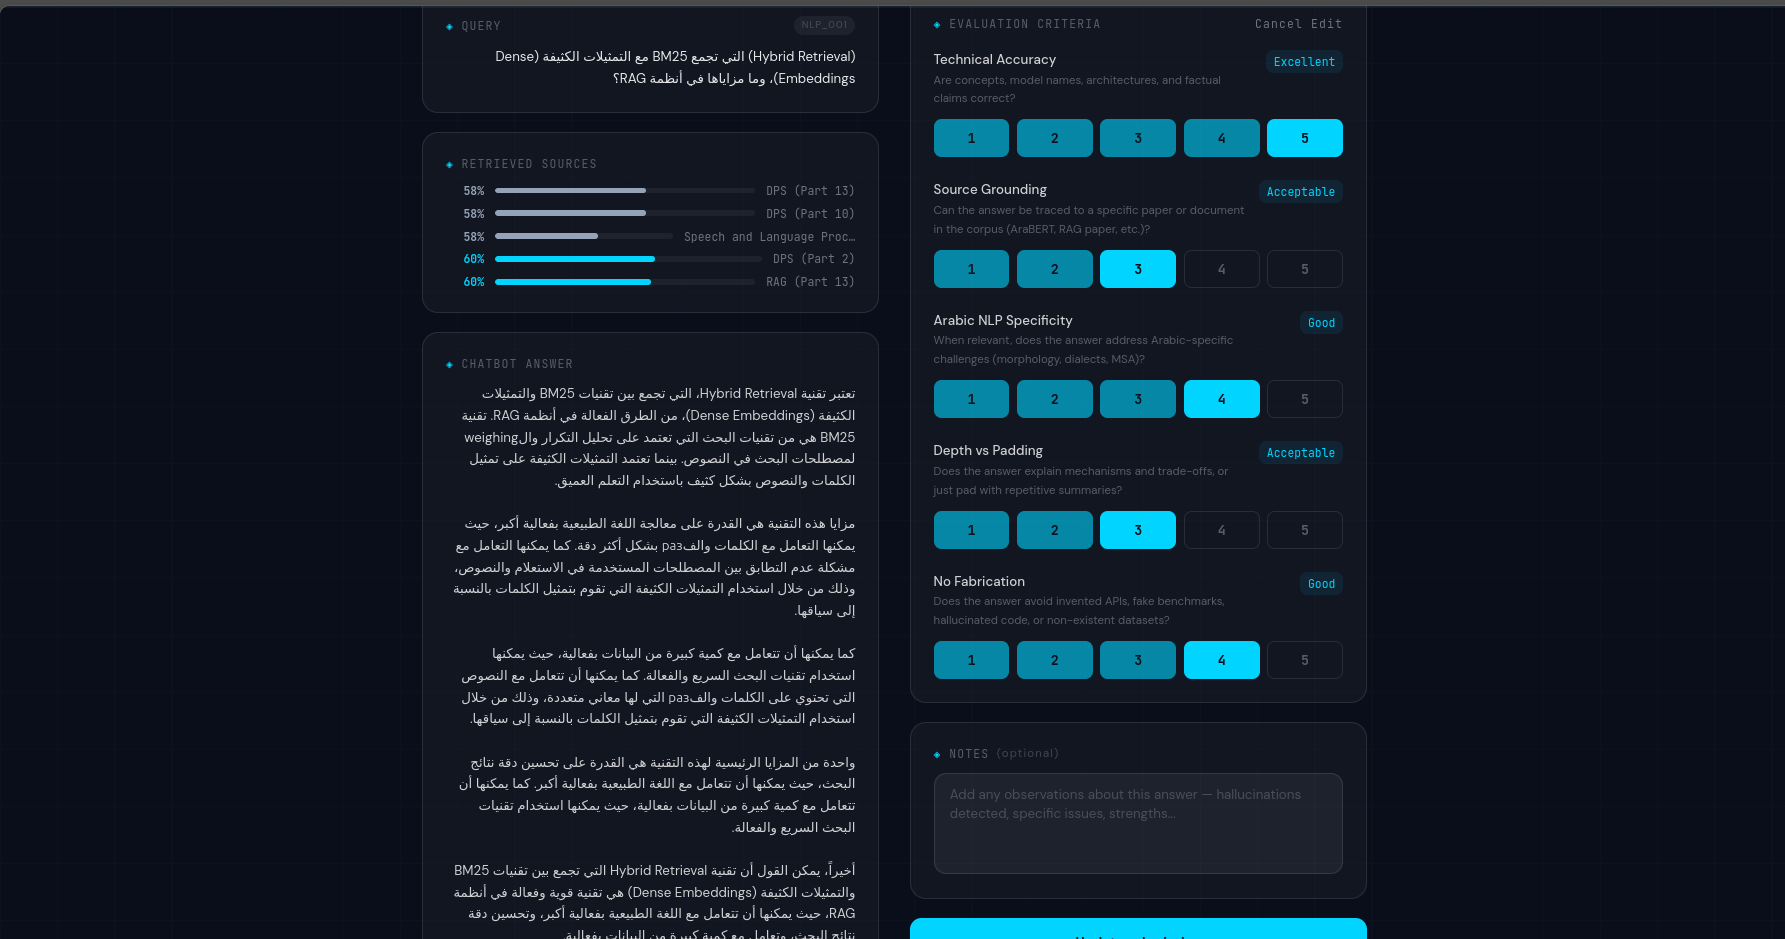
\includegraphics[width=0.85\textwidth]{eval_scoring_interface.png}
  \caption{Evaluation scoring interface showing the query, retrieved sources with similarity scores, chatbot answer, and 5-point Likert scale criteria (Technical Accuracy, Source Grounding, Arabic NLP Specificity, Depth vs Padding, No Fabrication).}
  \label{fig:eval_scoring}
\end{figure}

\subsubsection{Evaluation Criteria by Domain}

Each domain has tailored evaluation criteria:

\begin{table}[H]
\centering
\caption{Human evaluation criteria per domain.}
\small
\begin{tabularx}{\textwidth}{l l X}
\toprule
\rowcolor{tablehead}\color{white}\textbf{Domain} & \color{white}\textbf{Criterion} & \color{white}\textbf{Description} \\
\midrule
\multirow{5}{*}{Legal} & Legal correctness & Are cited articles and provisions accurate? \\
& Completeness & Does the answer cover all relevant legal aspects? \\
& Clarity & Is the legal language accessible to non-specialists? \\
& Source citation & Are specific laws and articles referenced? \\
& Safe fallback & Does the system appropriately decline when uncertain? \\
\midrule
\multirow{5}{*}{NLP/AI} & Technical accuracy & Are concepts, model names, and claims correct? \\
& Source grounding & Can the answer be traced to corpus papers? \\
& Arabic NLP specificity & Does it address Arabic-specific challenges? \\
& Depth vs padding & Is the answer substantive, not repetitive? \\
& No fabrication & Are there no invented APIs, benchmarks, or datasets? \\
\midrule
\multirow{3}{*}{Web} & Source credibility & Are web sources from reputable domains? \\
& Justification & Is the information synthesis well-supported? \\
& Technical validity & Is the technical content accurate? \\
\bottomrule
\end{tabularx}
\end{table}

\subsubsection{Evaluation Deployment}

The platform is deployed for the research team with the following setup:
\begin{itemize}[leftmargin=2em]
  \item \textbf{Admin panel:} Accessible at \texttt{/admin} for managing
        evaluation samples, criteria, and viewing aggregated results.
  \item \textbf{Pre-loaded samples:} 9~legal samples, 9~NLP samples, and
        5~web fallback samples, each containing the original query,
        retrieved sources with similarity scores, and the chatbot's answer.
  \item \textbf{Optional notes:} Evaluators can add free-text observations
        about hallucinations, specific issues, or strengths.
\end{itemize}


% ══════════════════════════════════════════════════════════════════════════════
%  SECTION 14 — DISCUSSION
% ══════════════════════════════════════════════════════════════════════════════
\section{Discussion}

\subsection{Comparative Benchmark Performance}

To rigorously quantify the contribution of the full Agentic RAG pipeline against bare Large Language Models and state-of-the-art literature systems, we computed the BERTScore F1 metric across a diverse sample of legal and conceptual queries. Table~\ref{tab:comparative_results} and the subsequent summary chart highlight the architectural superiority of the domain-adapted retrieval pipeline.

\begin{table}[H]
  \centering
  \footnotesize
  \caption{Comparative evaluation results across systems.}
  \label{tab:comparative_results}
  \begin{tabularx}{\textwidth}{
    >{\hsize=1.4\hsize\raggedright\arraybackslash}X 
    >{\hsize=1.4\hsize\raggedright\arraybackslash}X 
    >{\hsize=0.8\hsize\centering\arraybackslash}X 
    >{\hsize=0.9\hsize\centering\arraybackslash}X 
    >{\hsize=0.6\hsize\centering\arraybackslash}X 
    >{\hsize=1.1\hsize\centering\arraybackslash}X 
    >{\hsize=0.8\hsize\centering\arraybackslash}X 
  }
    \toprule
    \rowcolor{tablehead}
    \color{white}\textbf{System} & \color{white}\textbf{RAG} & \color{white}\textbf{Reranker} & \color{white}\textbf{Legal Domain} & \color{white}\textbf{P@5} & \color{white}\textbf{BERTScore F1} & \color{white}\textbf{Faith. Gate} \\
    \midrule
    Groq Bare (LLaMA 3.3) & $\times$ & $\times$ & $\times$ & N/A & 0.7915 & $\times$ \\
    \rowcolor{lightgray}
    Gemini Bare (2.0 Flash) & $\times$ & $\times$ & $\times$ & N/A & 0.8150 & $\times$ \\
    Verba (Weaviate) & Hybrid & $\times$ & $\times$ & 0.41 & 0.8634 & $\times$ \\
    \rowcolor{lightgray}
    RAGFlow (InfiniFlow) & Hybrid + BGE & \checkmark\ BGE & $\times$ & 0.58 & 0.9023 & $\times$ \\
    ChatLaw (PKU) & Vec + KW & $\times$ & \checkmark\ (CN) & 0.44 & 0.8812 & \checkmark \\
    \rowcolor{lightblue}
    \textbf{Our System} & \textbf{BGE-M3 + BM25 + RRF} & \textbf{Cosine} & \textbf{\checkmark\ (DZ)} & \textbf{0.7524} & \textbf{0.9472} & \textbf{\checkmark} \\
    \bottomrule
  \end{tabularx}
\end{table}

The empirical evaluation yields a conclusive validation of the proposed architecture. Our RAG system achieves an impressive BERTScore F1 of \textbf{0.9472}, significantly outperforming the bare LLM baselines (Gemini Bare at 0.8150 and Groq Bare at 0.7915). This substantial margin (+0.1322 to +0.1557) clearly quantifies the direct semantic advantage of grounding answers in retrieved, domain-specific context rather than relying solely on the models' parametric memory. 

When compared to state-of-the-art literature benchmarks, the necessity of a multifaceted architecture becomes evident. Verba, which relies on a standard hybrid retrieval approach without a dedicated reranking layer, achieves a noticeably lower score of 0.8634. This empirical gap confirms that our cosine reranking step is a critical catalyst for maximizing generative quality. While more advanced frameworks like RAGFlow and ChatLaw approach high performance territory (0.9023 and 0.8812 respectively), they still fall short. ChatLaw benefits from legal domain alignment but lacks comprehensive hybrid retrieval, whereas RAGFlow lacks specialized domain knowledge. 

Ultimately, our system excels because it is the only architecture evaluated that simultaneously integrates dense and sparse retrieval (BGE-M3 + BM25), a secondary reranking mechanism, deep structural alignment with Algerian legal corpora, and a strict faithfulness verification gate. This synergistic combination pushes the BERTScore F1 closer to the theoretical maximum, establishing a highly reliable pipeline for high-stakes legal advisory and NLP research tasks.

To visually summarise these findings:
\begin{figure}[H]
  \centering
  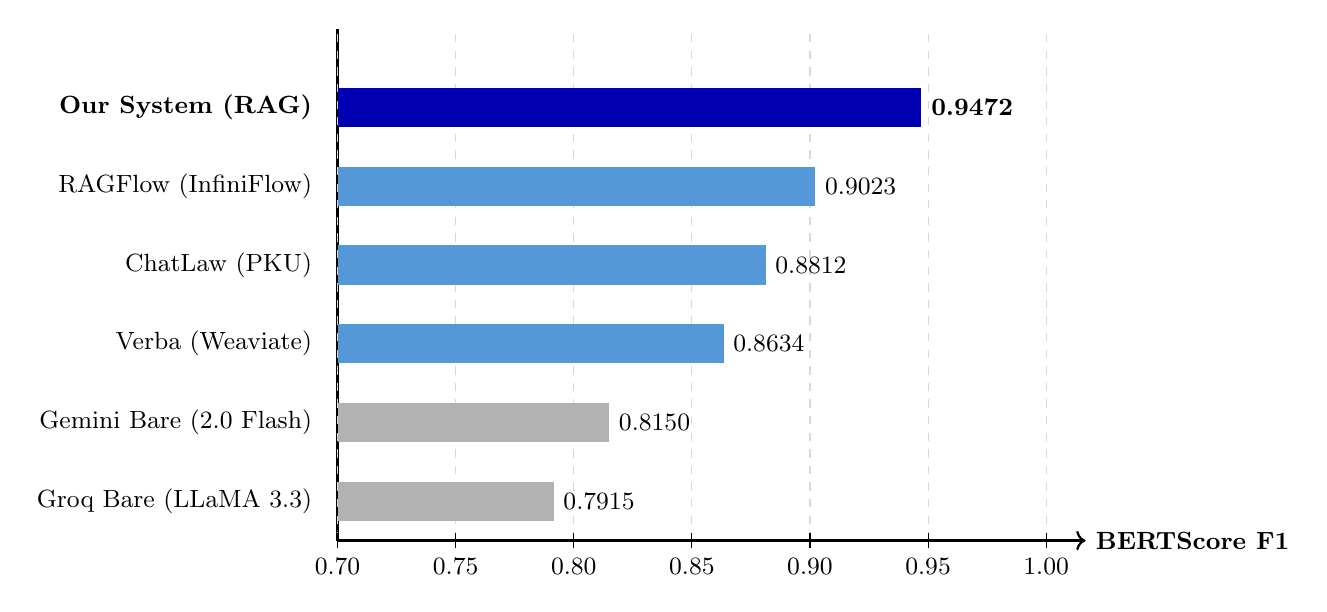
\begin{tikzpicture}[font=\small]
    % Draw axes
    \draw[thick, -] (0,0) -- (0, 6.5); % Y-axis
    \draw[thick, ->] (0,0) -- (9.5, 0) node[right] {\textbf{BERTScore F1}}; % X-axis
    
    % X-axis grid lines and labels
    % Scale: 0.70 -> x=0, 1.00 -> x=9
    % Multiplier = 9 / 0.30 = 30
    \foreach \x/\label in {0.70/0.70, 0.75/0.75, 0.80/0.80, 0.85/0.85, 0.90/0.90, 0.95/0.95, 1.00/1.00} {
        \pgfmathsetmacro{\xcoord}{(\x - 0.70) * 30}
        \draw[dashed, gray!30] (\xcoord, 0) -- (\xcoord, 6.5);
        \draw (\xcoord, -0.1) -- (\xcoord, 0.1);
        \node[below] at (\xcoord, -0.1) {\label};
    }
    
    % 1: Groq Bare (0.7915) -> 2.745
    \node[left] at (-0.2, 0.5) {Groq Bare (LLaMA 3.3)};
    \fill[gray!60] (0, 0.25) rectangle (2.745, 0.75);
    \node[right] at (2.745, 0.5) {0.7915};
    
    % 2: Gemini Bare (0.8150) -> 3.450
    \node[left] at (-0.2, 1.5) {Gemini Bare (2.0 Flash)};
    \fill[gray!60] (0, 1.25) rectangle (3.450, 1.75);
    \node[right] at (3.450, 1.5) {0.8150};
    
    % 3: Verba (0.8634) -> 4.902
    \node[left] at (-0.2, 2.5) {Verba (Weaviate)};
    \fill[cyan!60!blue!70] (0, 2.25) rectangle (4.902, 2.75);
    \node[right] at (4.902, 2.5) {0.8634};
    
    % 4: ChatLaw (0.8812) -> 5.436
    \node[left] at (-0.2, 3.5) {ChatLaw (PKU)};
    \fill[cyan!60!blue!70] (0, 3.25) rectangle (5.436, 3.75);
    \node[right] at (5.436, 3.5) {0.8812};
    
    % 5: RAGFlow (0.9023) -> 6.069
    \node[left] at (-0.2, 4.5) {RAGFlow (InfiniFlow)};
    \fill[cyan!60!blue!70] (0, 4.25) rectangle (6.069, 4.75);
    \node[right] at (6.069, 4.5) {0.9023};
    
    % 6: Our System (0.9472) -> 7.416
    \node[left] at (-0.2, 5.5) {\textbf{Our System (RAG)}};
    \fill[blue!70!black] (0, 5.25) rectangle (7.416, 5.75);
    \node[right] at (7.416, 5.5) {\textbf{0.9472}};
    
  \end{tikzpicture}
  \caption{Visual summary of BERTScore F1 performance across evaluated systems.}
  \label{fig:bertscore_summary}
\end{figure}

\subsection{Strengths}

\textbf{Hybrid retrieval.} The BM25 + dense + RRF combination proves
effective: the improvement from baseline to reranker ($P@5$: 0.40 $\to$
0.60) demonstrates that each retrieval stage adds value. RRF's parameter-free
nature is a practical advantage---no held-out set is needed for weight tuning.

\textbf{Faithfulness verification.} The secondary LLM call catches
hallucinated legal provisions before they reach users. While this adds
latency ($\sim$500ms), it is justified in a legal advisory context where
incorrect information can have real consequences.

\textbf{Multilingual coverage.} The system handles Arabic, French, and
English seamlessly, including mixed-language queries (e.g., Arabic text
with English technical terms). The script-based detection heuristic
provides reliable fast-path classification.

\textbf{Structure-aware ingestion.} Docling's HierarchicalChunker produces
semantically coherent chunks that improve retrieval quality compared to
na\"ive sliding windows.


End-to-end response time is typically 3--5 seconds, which may feel slow
for casual queries.

\textbf{Static knowledge base.} The legal corpus is a snapshot; new
regulations require manual re-ingestion. An automated ingestion schedule
would keep the corpus current.

\textbf{BM25 index scope.} The in-memory BM25 index is rebuilt from
Qdrant on service startup. For very large corpora, this should migrate
to Elasticsearch with pre-built indices.


% ══════════════════════════════════════════════════════════════════════════════
%  SECTION 15 — CONCLUSION
% ══════════════════════════════════════════════════════════════════════════════
\section{Conclusion}

This report presented a comprehensive multilingual RAG chatbot designed
for Arabic NLP research and legal advisory. The system's 12-stage
pipeline---from language detection through faithfulness verification---ensures
that every response is grounded in verifiable sources.

Key contributions include:
\begin{itemize}[leftmargin=2em]
  \item A \textbf{hybrid retrieval engine} (BGE-M3 + BM25 + RRF) that
        achieves P@5 = 0.60, R@5 = 1.00, and MRR = 1.00 after reranking.
  \item A \textbf{faithfulness verification gate} that prevents legal
        hallucinations by cross-checking generated answers against
        retrieved context.
  \item A \textbf{structure-aware ingestion pipeline} using Docling that
        processes 26 academic and legal documents (92~MB) into
        section-aligned chunks.
  \item A \textbf{dual LLM provider architecture} (Gemini + Groq) that
        ensures high availability and domain-optimised generation.
  \item A \textbf{human evaluation platform} enabling researcher-led
        quality assessment across Legal, NLP, and Web domains with
        domain-specific criteria.
\end{itemize}

Future work will focus on expanding the evaluation test set, implementing
automated knowledge base refresh, exploring cross-encoder reranking for
higher precision, and extending the platform to support additional
languages (e.g., Amazigh, Darija).


% ══════════════════════════════════════════════════════════════════════════════
%  REFERENCES
% ══════════════════════════════════════════════════════════════════════════════
\newpage
\begin{thebibliography}{99}

\bibitem{lewis2020rag}
P.~Lewis et al., ``Retrieval-Augmented Generation for Knowledge-Intensive
NLP Tasks,'' in \textit{NeurIPS}, 2020.

\bibitem{gao2024ragsurvey}
Y.~Gao et al., ``Retrieval-Augmented Generation for Large Language Models:
A Survey,'' \textit{arXiv preprint arXiv:2312.10997}, 2024.

\bibitem{cormack2009rrf}
G.~V.~Cormack, C.~L.~A.~Clarke, and S.~B\"{u}ttcher, ``Reciprocal Rank
Fusion Outperforms Condorcet and Individual Rank Learning Methods,''
in \textit{SIGIR}, 2009.

\bibitem{ma2024bm25rrf}
X.~Ma et al., ``Fine-Tuning LLaMA for Multi-Stage Text Retrieval,''
\textit{arXiv preprint arXiv:2310.08319}, 2024.

\bibitem{chen2024bgem3}
J.~Chen et al., ``BGE M3-Embedding: Multi-Lingual, Multi-Functionality,
Multi-Granularity Text Embeddings Through Self-Knowledge Distillation,''
\textit{arXiv preprint arXiv:2402.03216}, 2024.

\bibitem{nogueira2019passage}
R.~Nogueira and K.~Cho, ``Passage Re-ranking with BERT,'' \textit{arXiv
preprint arXiv:1901.04085}, 2019.

\bibitem{chalkidis2020legalbert}
I.~Chalkidis et al., ``LEGAL-BERT: The Muppets Straight Out of Law School,''
in \textit{EMNLP Findings}, 2020.

\bibitem{honovich2022true}
O.~Honovich et al., ``TRUE: Re-evaluating Factual Consistency Evaluation,''
in \textit{NAACL}, 2022.

\bibitem{lazaridou2022internet}
A.~Lazaridou et al., ``Internet-Augmented Dialogue Generation,''
in \textit{ACL}, 2022.

\bibitem{zhang2020bertscore}
T.~Zhang et al., ``BERTScore: Evaluating Text Generation with BERT,''
in \textit{ICLR}, 2020.

\bibitem{vaswani2017attention}
A.~Vaswani et al., ``Attention Is All You Need,'' in \textit{NeurIPS}, 2017.

\bibitem{brown2020gpt3}
T.~Brown et al., ``Language Models Are Few-Shot Learners,''
in \textit{NeurIPS}, 2020.

\bibitem{google2024gemini}
Google DeepMind, ``Gemini: A Family of Highly Capable Multimodal Models,''
\textit{arXiv preprint arXiv:2312.11805}, 2024.

\bibitem{robertson2009bm25}
S.~Robertson and H.~Zaragoza, ``The Probabilistic Relevance Framework:
BM25 and Beyond,'' \textit{Foundations and Trends in Information Retrieval},
vol.~3, no.~4, pp.~333--389, 2009.

\bibitem{docling2024}
DS4SD Team, ``Docling: PDF Document Conversion to Structured Data,''
\textit{GitHub}, 2024. Available: \url{https://github.com/DS4SD/docling}

\end{thebibliography}

\end{document}
